% CVPR 2027 Supplementary Material — full proofs and numerics
\documentclass[10pt,letterpaper]{article}

\usepackage{cvpr}

%% Preamble: kit defaults + project additions

%% Official support for 2-column teaser figure
\usepackage{cuted} %< for strip environment

%% For auto-referencing of figures
\usepackage{currfile} %< for \currfilebase macro

%% caption support for teaser
\usepackage{caption}

%% Inline annotations
\newcommand{\red}[1]{{\color{red}#1}}
\newcommand{\todo}[1]{{\color{red}#1}}
\newcommand{\TODO}[1]{\textbf{\color{red}[TODO: #1]}}
%% Disable for camera ready / submission by uncommenting these lines:
% \renewcommand{\TODO}[1]{}
% \renewcommand{\todo}[1]{#1}

%% ---------- Project additions ----------
\usepackage{amsmath}
\usepackage{amssymb}
\usepackage{amsthm}
\usepackage{booktabs}
\usepackage{graphicx}
\usepackage{subcaption}
\usepackage{multirow}

\newtheorem{theorem}{Theorem}
\newtheorem{corollary}[theorem]{Corollary}
\newtheorem{lemma}[theorem]{Lemma}
\newtheorem{proposition}[theorem]{Proposition}
\theoremstyle{definition}
\newtheorem{assumption}{Assumption}
\theoremstyle{remark}
\newtheorem{remark}{Remark}

%% Notation macros
\newcommand{\R}{\mathbb{R}}
\newcommand{\E}{\mathbb{E}}
\newcommand{\risk}{\mathcal{R}_T}        % robot-domain excess risk
\newcommand{\riske}{\bar{\mathcal{R}}_T} % deterministic equivalent
\newcommand{\lead}{\mathrm{lead}}         % leading-order risk object
\newcommand{\nr}{n_r}
\newcommand{\nh}{n_h}
\newcommand{\kex}{\kappa_{\mathrm{ex}}}  % ego<->teleop exchange rate


\definecolor{cvprblue}{rgb}{0.21,0.49,0.74}
\usepackage[pagebackref,breaklinks,colorlinks,allcolors=cvprblue]{hyperref}

\def\paperID{*****} % *** Enter the Paper ID here
\def\confName{CVPR}
\def\confYear{2027}

\title{Supplementary Material for\\
When Does Auxiliary Data Help? Spectral Risk and\\
Optimal Mixing under Task Mismatch}

\author{Anonymous \confName~\confYear~submission\\
Paper ID \paperID
}

\begin{document}
\maketitle
\appendix
%% Supplementary material — full version (compiled as suppl.pdf via suppl.tex)
%% Self-contained: restates the model and all equations used.

The supplement follows the main text's global-mixing hierarchy: full-ridge risk and derivative expansions lead to the interior optimum and matched-spectrum gain expansion. A first-order exchange equation and an exact dosage solution for a quadratic surrogate are stated separately. Diagonalized leading-order identities and boundary cases are included as special cases and counterexamples, not as the main narrative. Throughout, C1 refers to the marginal-benefit decomposition and C2 to the diagonalized marginal criterion.

\begin{table}[h]
  \centering
  \small
  \caption{Claim--object map. Exact identities for the diagonalized leading-order object are separate from asymptotic expansions of the actual full-ridge risk.}
  \label{supp:tab:claimobjects}
  \begin{tabular}{@{}p{.17\linewidth}p{.29\linewidth}p{.42\linewidth}@{}}
    \toprule
    Result & Estimator and risk object & Established scope \\
    \midrule
    T1-a & Diagonalized; leading order & Conditional per-coordinate approximation, not an exact finite-sample identity \\
    C1, C2 & Diagonalized; $\riske^{\lead}$ & Exact marginal decomposition and critical-size algebra for this object \\
    Exchange rate, dosage & Diagonalized; $\riske^{\lead}$ & Full-interval optimization under the stated baseline and spectral conditions \\
    T1-c, full derivative & Standard full ridge; actual risk & Fixed-$p$ second-order risk and uniform first/second derivatives; zero-mixing expansion is a special case \\
    Interior optimum & Standard full ridge; actual risk & First-order optimal-weight correction and optimized risk/gain expansions at a unique nondegenerate interior population minimizer; no boundary-switching claim \\
    Boundary optima & Standard full ridge; actual risk & Nondegenerate boundary persistence and flat-boundary weight/gain rates; local--global counterexample included \\
    Matched gain, exchange & Full ridge; matched spectra & Optimized-gain expansion and exchange equation based on first-order risks \\
    Surrogate dosage & Population-plus-noise quadratic & Exact piecewise optimum of this surrogate; no full-ridge dosage guarantee \\
    \bottomrule
  \end{tabular}
\end{table}

\section{Setup and notation}
\label{supp:setup}

We restate the model of the main text (Sec.~3) for self-containment.
Coordinates $j = 1,\dots,p$ index a shared spectral basis; domain $e \in \{r, h\}$ has covariates $x_e = \Sigma_e^{1/2} u_e$, $u_e$ standard Gaussian, $\Sigma_e = \mathrm{diag}(\lambda^e_j)$ with $\lambda^e_j \asymp j^{-\alpha_e}$, $\lambda^e_1 = 1$; we write $a_j = \lambda^r_j$, $b_j = \lambda^h_j$.
Labels: $y_r = \langle\beta^*, x_r\rangle + \varepsilon_r$, $y_h = \langle\beta^* + \delta, x_h\rangle + \varepsilon_h$; $\sum_j j^{2s}\beta_j^{*2} \le 1$; noise variances $\sigma_e^2$.
Given $\nr$ robot and $\nh$ human samples, mixing ratio $\lambda \in [0,1]$, per-sample weights $w_r = (1-\lambda)/\nr$, $w_h = \lambda/\nh$, the diagonalized ridge estimator is
\begin{equation}
\begin{aligned}
  \hat\beta_j &= \frac{w_r T_{rj} + w_h T_{hj}}{w_r S_{rj} + w_h S_{hj} + \mu},\\
  S_{ejk} &= {\textstyle\sum_{i=1}^{n_e}} x_{e,ij} x_{e,ik},\qquad
  T_{ej} = {\textstyle\sum_i} x_{e,ij}\, y_{e,i}.
\end{aligned}
  \label{supp:eq:estimator}
\end{equation}
The robot-domain excess risk is $\risk(\lambda) = \E\|\hat\beta(\lambda) - \beta^*\|^2_{\Sigma_r} = \sum_j a_j\, \E(\hat\beta_j - \beta^*_j)^2$.
The effective noise is $\tilde\sigma_{e,j}^2 = \sigma_e^2 + F_{e,j}$ with per-coordinate feedthrough energy $F_{e,j} = \sum_{k\neq j} \lambda^e_k \beta_{e,k}^2$ ($\beta_h = \beta^* + \delta$); where the coordinate dependence is immaterial we abbreviate $\tilde\sigma_{e,j}^2$ (resp.\ $F_{e,j}$) as $\tilde\sigma_e^2$ (resp.\ $F_e$), and all numerical evaluations use the exact per-coordinate form.

\medskip
\noindent\textbf{Single-coordinate notation} (used throughout, index $j$ suppressed).
$U_r \sim \chi^2_{\nr}$, $U_h \sim \chi^2_{\nh}$ independent; $S_e = \lambda^e U_e$, so $\E S_e = n_e\lambda^e$, $\mathrm{Var}(S_e) = 2n_e(\lambda^e)^2$, and the third central moment is $8n_e(\lambda^e)^3$.
$\hat D = w_r S_r + w_h S_h + \mu$; $D = \E\hat D = (1-\lambda)a + \lambda b + \mu$.
$\hat N = w_r T_{r} + w_h T_{h}$; its systematic part $N_0 = \lambda b\,\delta - \mu\beta^*$.
The fluctuation scale is $\eta = \sqrt{8\log(4p/\delta_c)}\,\big(\frac{(1-\lambda)a}{\sqrt{\nr}} + \frac{\lambda b}{\sqrt{\nh}}\big)$ for confidence parameter $\delta_c \in (0,1)$.
We write $\tilde n = \hat N - \E\hat N$; direct expansion gives
\begin{equation}
  \mathrm{Var}(\tilde n) = \underbrace{\frac{2\lambda^2 (b\delta)^2}{\nh}}_{\text{mismatch fluctuation}} + \underbrace{\frac{(1{-}\lambda)^2 \tilde\sigma_r^2 a}{\nr} + \frac{\lambda^2 \tilde\sigma_h^2 b}{\nh}}_{\text{noise + feedthrough}} .
  \label{supp:eq:varn}
\end{equation}

\section{Lemmas L1 and L2: per-coordinate representation and conditional MSE}
\label{supp:l12}

\begin{lemma}[L1, representation]\label{supp:l1}
For each coordinate $j$, with the definitions above,
\begin{equation}
  T_{ej} = S_{ejj}\,\beta_{e,j} + U_{ej} + \textstyle\sum_i x_{e,ij}\varepsilon_{e,i},
  \qquad U_{ej} = \sum_{k\neq j} S_{ejk}\,\beta_{e,k},
  \label{supp:eq:l1}
\end{equation}
where $U_{ej}$ is mean-zero with $\mathrm{Var}(U_{ej}) = n_e \lambda^e_j F_{e,j}$, $F_{e,j} = \sum_{k\neq j} \lambda^e_k \beta_{e,k}^2$.
\end{lemma}

\begin{proof}
Expand $y_{e,i} = \sum_k x_{e,ik}\beta_{e,k} + \varepsilon_{e,i}$ in $T_{ej} = \sum_i x_{e,ij} y_{e,i}$ and separate the $k = j$ term.
For $k \neq j$, $\E S_{ejk} = \sum_i \E[x_{e,ij}]\E[x_{e,ik}] = 0$ by independence of distinct coordinates of the Gaussian covariate, hence $\E U_{ej} = 0$.
For the variance, $\mathrm{Var}(S_{ejk}) = \sum_i \E[x_{e,ij}^2]\E[x_{e,ik}^2] = n_e \lambda^e_j \lambda^e_k$ (independence of coordinates $j \neq k$), and distinct cross terms are uncorrelated: for $k \neq l$, $\mathrm{Cov}(S_{ejk}, S_{ejl}) = \sum_i \E[x_{e,ij}^2 x_{e,ik} x_{e,il}] = 0$ since $\E[x_{e,ik}x_{e,il}] = 0$ and $x_{e,ij}^2$ is independent of $(x_{e,ik}, x_{e,il})$.
Summing, $\mathrm{Var}(U_{ej}) = \sum_{k\neq j} \beta_{e,k}^2 \, n_e \lambda^e_j \lambda^e_k = n_e \lambda^e_j F_{e,j}$.
We retain the exact per-coordinate form $F_{e,j}$ throughout; no approximation of $F_{e,j}$ by the total signal energy $\sum_k \lambda^e_k\beta_{e,k}^2$ is made, since the omitted single term need not be negligible --- for a low-frequency-concentrated $\beta^*$ (the regime of the ellipsoid constraint in the main text), the first coordinates can carry an $O(1)$ fraction of the total energy.
\end{proof}

\begin{remark}
The feedthrough $U_{ej}$ contributes variance $n_e\lambda^e_j F_{e,j}$ to the coordinate-$j$ numerator, which motivates the effective noise $\tilde\sigma_{e,j}^2$ in Eq.~\eqref{supp:eq:varn}. This is a variance calculation only: $U_{ej}$ and $S_{ejj}$ share $x_{e,ij}$ and are not independent. In fact, $\operatorname{Var}(U_{ej}\mid X_{e,:j})=F_{e,j}S_{ejj}$. Higher-moment arguments must not treat them as independent.
\end{remark}

\begin{lemma}[L2, conditional MSE]\label{supp:l2}
Define $N_{0j}^{X}=w_hS_{hjj}\delta_j-\mu\beta^*_j+w_rU_{rj}+w_hU_{hj}$, which is deterministic conditional on $X$. Then
\begin{align}
  \E\big[(\hat\beta_j-\beta^*_j)^2\mid X\big]
  &=\frac{(N_{0j}^{X})^2}{\hat D_j^2}
  +\frac{w_r^2\sigma_r^2S_{rjj}}{\hat D_j^2}
  +\frac{w_h^2\sigma_h^2S_{hjj}}{\hat D_j^2}.
  \label{supp:eq:l2}
\end{align}
\end{lemma}

\begin{proof}
Substitute Lemma~\ref{supp:l1} into Eq.~\eqref{supp:eq:estimator}:
$\hat\beta_j \hat D_j = w_r S_{rjj}\beta^*_j + w_h S_{hjj}(\beta^*_j + \delta_j) + (\text{feedthrough} + \text{noise})$.
Subtract $\beta^*_j \hat D_j = w_r S_{rjj}\beta^*_j + w_h S_{hjj}\beta^*_j + \mu\beta^*_j$. The systematic numerator is $N_{0j}^{X}$. The remaining zero-mean label-noise projection is $w_rX_{r,:j}^\top\varepsilon_r+w_hX_{h,:j}^\top\varepsilon_h$. Its conditional variance is $w_r^2\sigma_r^2S_{rjj}+w_h^2\sigma_h^2S_{hjj}$, and cross terms vanish by independence and zero mean.
\end{proof}

\section{Lemma L3: leading per-coordinate approximation}
\label{supp:l3}

\begin{lemma}[L3, leading order]\label{supp:l3lem}
Fix a coordinate and suppose $D \ge 2\eta$ (information-rich regime).
Define
\begin{align}
  \mathrm{MSE}^{\lead} &= \frac{N_0^2 + \mathrm{Var}(\tilde n)}{D^2}, \notag\\
  \overline N^2 &= N_0^2 + \mathrm{Var}(\tilde n),
  \qquad M_4=(\E\hat N^4)^{1/2}.
  \label{supp:eq:mselead}
\end{align}
Then
\begin{align}
  \left|\E\!\left[\frac{\hat N^2}{\hat D^2}\right]-\mathrm{MSE}^{\lead}\right|
  &\le C\frac{\eta}{D}\frac{M_4}{D^2}
  +O\!\left(\frac{\eta^2}{D^2}\frac{\overline N^2}{D^2}\right) \notag\\
  &\quad+O\!\left(\sqrt{\delta_c}\,\mu^{-2}M_4\right),
  \label{supp:eq:l3bound}
\end{align}
where $C$ is an absolute constant and $M_4$ is finite under the Gaussian design and the noise moment assumptions.
\end{lemma}

\begin{proof}
\emph{Step 1 (concentration).}
Write $\Delta=\hat D-D$. By the Laurent--Massart $\chi^2$ tail bound and a union bound, there is an event $G$ with $\Pr(G)\ge1-\delta_c$ on which $|\Delta|\le\eta\le D/2$ simultaneously for all retained coordinates. Also, $\E\Delta^2=O(\eta^2)$.

\emph{Step 2 (Taylor expansion on $G$).}
For $f(x)=x^{-2}$,
\begin{equation}
  f(D+\Delta)=D^{-2}-2\Delta D^{-3}+R,
  \qquad |R|\le48\eta^2/D^4 .
  \label{supp:eq:taylorlead}
\end{equation}
Splitting the expectation into good and bad events gives
\begin{align}
  \E[\hat N^2f(\hat D)]
  &=\E[\hat N^2f(\hat D)\mathbf 1_G]
  +\E[\hat N^2f(\hat D)\mathbf 1_{G^c}] \notag\\
  &=D^{-2}\E\hat N^2
  -2D^{-3}\E[\hat N^2\Delta\mathbf 1_G] \notag\\
  &\quad+\E[\hat N^2R\mathbf 1_G]
  +\E[\hat N^2f(\hat D)\mathbf 1_{G^c}].
  \label{supp:eq:eventdecomp}
\end{align}
The difference from $\overline N^2/D^2$ therefore contains four terms: the subtracted $D^{-2}\E[\hat N^2\mathbf 1_{G^c}]$, the cross term $-2D^{-3}\E[\hat N^2\Delta\mathbf 1_G]$, the Taylor remainder $\E[\hat N^2R\mathbf 1_G]$, and the actual bad-event risk $\E[\hat N^2f(\hat D)\mathbf 1_{G^c}]$.

Cauchy--Schwarz gives
\begin{align}
  |\E[\hat N^2\Delta\mathbf 1_G]|
  &\le (\E\hat N^4)^{1/2}(\E\Delta^2)^{1/2} \notag\\
  &=O(\eta M_4).
  \label{supp:eq:crosslead}
\end{align}
The Taylor term is at most $48\eta^2\overline N^2/D^4$. No independence between feedthrough and $\hat D$ is used.

\emph{Step 3 (both complementary-event terms).}
Since $\hat D\ge\mu>0$, another Cauchy--Schwarz bound yields
\begin{align}
  D^{-2}\E[\hat N^2\mathbf 1_{G^c}]
  &\le D^{-2}\sqrt{\delta_c}\,M_4, \notag\\
  \E[\hat N^2f(\hat D)\mathbf 1_{G^c}]
  &\le \mu^{-2}\sqrt{\delta_c}\,M_4.
  \label{supp:eq:badlead}
\end{align}
Combining the four terms proves Eq.~\eqref{supp:eq:l3bound}; the first two are controlled by $C(\eta/D)M_4/D^2$ because $\eta/D\le1/2$.
\end{proof}

\paragraph{A corrected numerical surrogate, not a second-order theorem.}
For computation, we also evaluate
\begin{align}
  \mathrm{MSE}^{\det}
  &= \mathrm{MSE}^{\lead}
  -\frac{4N_0\mathrm{Cov}(\tilde n,\hat D)}{D^3} \notag\\
  &\quad+\frac{3N_0^2\mathrm{Var}(\hat D)}{D^4},
  \label{supp:eq:msedet}
\end{align}
with $\mathrm{Cov}(\tilde n,\hat D)=2\lambda^2\delta b^2/\nh$ and $\mathrm{Var}(\hat D)=2[(1-\lambda)^2a^2/\nr+\lambda^2b^2/\nh]$. This is a delta-method-inspired numerical surrogate. It is not covered by Lemma~\ref{supp:l3lem}: feedthrough and the denominator are dependent, and the mixed moments and higher-order terms required for a uniform corrected error bound are not asserted to be controlled. In particular, we do not claim that the mixed moment $\E[\tilde n^2\Delta]$ or all higher-order numerator terms vanish.

\section{Aggregation and truncation scope}
\label{supp:l4}

No global truncation lemma is asserted under Assumptions~A1--A3. The ellipsoid constraint $\sum_j j^{2s}\beta_j^{*2}\le1$ does not imply a coordinatewise law $\beta_j^{*2}\asymp j^{-(2s+1)}$ or a two-sided power-law tail. It permits sparse and concentrated task vectors.
Moreover, a truncated coordinate can have $\beta_j^*=0$ but $\delta_j\ne0$, in which case human data can produce nonzero bias and variance; its risk cannot be $\Theta(\beta_j^{*2})$. Even with zero mismatch, noise can prevent such an equivalence.
Consequently, we do not claim a global error bound obtained by replacing the tail with $\sum_{j>m}a_j\beta_j^{*2}$, nor do we assert a tail rate or a boundary-band cardinality without additional assumptions. A global approximation to the true total risk requires separate control of task mismatch, noise, and the information-poor coordinates.

\section{Two deterministic risk objects and the scope of exact identities}
\label{supp:riskobjects}

Define the leading-order and corrected per-coordinate risks by
\begin{align}
  \mathrm{MSE}^{\lead} &:= \frac{N_0^2+\mathrm{Var}(\tilde n)}{D^2}, \notag\\
  \mathrm{MSE}^{\det} &= \mathrm{MSE}^{\lead}
  -\frac{4N_0\mathrm{Cov}(\tilde n,\hat D)}{D^3} \notag\\
  &\qquad +\frac{3N_0^2\mathrm{Var}(\hat D)}{D^4}.
  \label{supp:eq:lead-det}
\end{align}
The leading numerator includes the mismatch-fluctuation term in Eq.~\eqref{supp:eq:varn}.
Aggregating the per-coordinate expressions over the explicitly specified retained set in each protocol defines the formal objects $\riske^{\lead}$ and $\riske^{\det}$, respectively. These are deterministic risk objects used for analysis and computation, not a proved truncation approximation to the true total risk.
All structural identities below (the marginal decomposition, the $H$ criterion, unimodality, the matched-spectrum quadratic form, the exchange rate, and the dosage law) concern $\riske^{\lead}$.
The L3 leading-order approximation concerns $\riske^{\lead}$; corrected numerical risk curves use the surrogate $\riske^{\det}$.

\begin{proposition}[explicit derivative correction at zero mixing]
\label{supp:prop:derivcorr}
Write $u=b\delta$, $w=\mu\beta^*$, and $D_0=a+\mu$. Then, coordinate by coordinate,
\begin{align}
  \partial_\lambda\mathrm{MSE}^{\det}\big|_{0^+}
  &=\partial_\lambda\mathrm{MSE}^{\lead}\big|_{0^+}
  -\frac{12a^2w(u+w)}{\nr D_0^4} \notag\\
  &\qquad -\frac{24a^2w^2(b-a)}{\nr D_0^5}.
  \label{supp:eq:derivcorr}
\end{align}
The covariance correction contributes zero at $\lambda=0$.
The aggregate correction is obtained by multiplying the displayed terms by $a_j$ and summing over retained coordinates.
\end{proposition}

\begin{proof}
Put $C(\lambda)=\mathrm{Cov}(\tilde n,\hat D)=2\lambda^2\delta b^2/\nh$ and $W(\lambda)=\mathrm{Var}(\hat D)=2[(1-\lambda)^2a^2/\nr+\lambda^2b^2/\nh]$.
Since $C(0)=C'(0)=0$, differentiating $-4N_0C/D^3$ at zero gives no contribution.
Moreover $N_0(0)=-w$, $N_0'(0)=u$, $W(0)=2a^2/\nr$, $W'(0)=-4a^2/\nr$, and $D'(0)=b-a$.
Differentiating $3N_0^2W/D^4$ and substituting these values gives Eq.~\eqref{supp:eq:derivcorr}.
\end{proof}

Thus the correction is $O(\nr^{-1})$ per coordinate and vanishes when $\nr\to\infty$ with $\nh/\nr$ fixed: the asymptotic functional $H$ is unchanged.
Finite-$\nr$ statements such as $\nr^{\mathrm{crit}}=K/H$ are exact for $\riske^{\lead}$; for $\riske^{\det}$ the additional terms in Eq.~\eqref{supp:eq:derivcorr} must be included instead of treating $K$ as correction-free.
Likewise, at matched spectra $N_0$ is affine and $C,W$ are quadratic, so $\mathrm{MSE}^{\det}$ generally contains cubic and quartic terms in $\lambda$.
The exact quadratic and hyperbolic dosage identities below therefore apply to $\riske^{\lead}$, not to $\riske^{\det}$ or to the unapproximated finite-sample risk.

\section{Proof of the marginal-benefit decomposition (C1)}
\label{supp:c1}

Differentiate the leading-order expression in Eq.~\eqref{supp:eq:lead-det} at $\lambda = 0^+$ per coordinate.
With $D_0 = a + \mu$, $V = \tilde\sigma_{r,j}^2 a/\nr$, direct expansion gives
\begin{equation}
  \partial_\lambda \mathrm{MSE}^{\lead}\big|_{0^+} = \frac{-2\mu\beta^* b\, \delta - 2V}{D_0^2} - \frac{2\big(V + \mu^2\beta^{*2}\big)(b - a)}{D_0^3},
  \label{supp:eq:c1deriv}
\end{equation}
which, after flipping the sign and dropping the positive factor $2/D_0^3$, is the three-term decomposition of the main text:
\begin{equation}
  \mathrm{benefit}_j \;\propto\; \underbrace{\mu\beta^*_j b_j \delta_j D_{0j}}_{\text{A: alignment}} + \underbrace{V_j D_{0j}}_{\text{B: variance}} + \underbrace{\big(V_j + \mu^2\beta_j^{*2}\big)(b_j - a_j)}_{\text{C: coverage}} .
  \label{supp:eq:c1}
\end{equation}
Analytic derivative vs.\ finite differences on the leading-order formula: relative error $<1\%$ (configuration of the v2 benchmark).
The derivative of $\mathrm{MSE}^{\det}$ has the additional explicit terms of Proposition~\ref{supp:prop:derivcorr}.
At $\mu = 0$, $D_0 = a$, terms A and the shrinkage part of C vanish, and
$\partial_\lambda\riske^{\lead}(0^+)|_{\mu=0} = -(2/\nr)\sum_j \tilde\sigma_{r,j}^2 b_j/a_j < 0$ always. For exact power-law spectra and coordinate-invariant effective noise, this reduces to $-(2\tilde\sigma_r^2/\nr)\sum_j j^{\alpha_r-\alpha_h}$.

\section{The central $H$-criterion: derivation and scope}
\label{supp:h}

Take $\nr \to \infty$ with $\nh/\nr$ fixed in Eq.~\eqref{supp:eq:c1deriv}: the variance term B vanishes, and the zero-mixing risk derivative converges to $H$ (equivalently, the marginal benefit converges to $-H$), for a general mismatch vector:
\begin{equation}
  H = \underbrace{-2\mu \sum_j \frac{a_j\beta^*_j b_j \delta_j}{D_{0j}^2}}_{A_\infty} - \underbrace{2\mu^2 \sum_j \frac{a_j\beta_j^{*2}(b_j - a_j)}{D_{0j}^3}}_{C_\infty}.
  \label{supp:eq:h}
\end{equation}
At finite $\nr$ the variance terms of $\riske^{\lead}$ contribute $-K/\nr$ to the derivative, with $K = 2\sum_j\tilde\sigma_{r,j}^2(S_{1j} + S_{2j})$, $S_{1j} = a_j^2/D_{0j}^2$, $S_{2j} = a_j^2(b_j-a_j)/D_{0j}^3$; hence marginal mixing is beneficial iff $K/\nr > H$, giving $\nr^{\mathrm{crit}} = K/H$ when $H > 0$. Here $S_{1j}+S_{2j}=a_j^2(b_j+\mu)/D_{0j}^3>0$, so $K>0$ whenever $\tilde\sigma_{r,j}^2>0$.
Proposition~\ref{supp:prop:derivcorr} vanishes in this large-$\nr$ limit, so $H$ is unchanged for $\riske^{\det}$; the displayed finite-$\nr$ formula is exact for $\riske^{\lead}$, with the stated correction required for $\riske^{\det}$.
Under the experimental convention $\beta_j^*>0$ and $\delta_j=-z_j$ with $z_j\ge0$, the signed first term reduces to $2\mu\sum_j a_j\beta_j^*b_jz_j/D_{0j}^2$; hence the anti-aligned numerical configurations also satisfy the earlier absolute-value specialization.
Numerically (v11, $p = 1000$, $\mu = 0.05$, spectral family A): $A_\infty$ is linear in $\|\delta\|$ with slope $6.975\times10^{-3}$, $C_\infty = 4.700\times10^{-3}$ independent of $\delta$, predicting $\|\delta\|^* = 0.674$, which brackets the sign change of the analytic/numerical risk derivative; and $\nr^{\mathrm{crit}}\cdot H = 25.866$ is constant across $\|\delta\| \in \{0.75, 1.0, 2.0\}$ to display precision when both sides are computed from the same leading-order formula.
These v11 checks are algebraic/numerical self-consistency, not independent Monte-Carlo phase validation.

\paragraph{The classical limit and its order of limits.}
At fixed finite dimension, $H=O(\mu)$ as $\mu\to0$, and if $A_\infty>0$ then $\nr^{\mathrm{crit}}=K/H\to\infty$.
Thus, at any fixed $\nr$, sufficiently small $\mu$ gives $K/\nr>H$ and marginal mixing is beneficial, consistently with the $\mu=0$ identity above.
The discard-the-source transition is recovered only when $\nr$ crosses the threshold as $\mu$ decreases (asymptotically $\nr\gtrsim1/\mu$, with constants determined by $K/A_\infty$); it is not obtained by taking $\mu\to0$ at fixed $\nr$.
At fixed $\mu > 0$ the large-$\nr$ marginal mixing benefit tends to $-A_\infty+C_\infty=-H$: when $H<0$, regularization preserves a positive coverage benefit even with unlimited robot data.

\section{Consequences: exchange rate, unimodality, and dosage}
\label{supp:t2}

Throughout this section $\riske$ denotes $\riske^{\lead}$; the denominator-fluctuation corrections of $\riske^{\det}$ are not part of these algebraic identities.
The exchange rate is defined implicitly by $\riske(\lambda^*;\, \nr, \nh) = \riske(0;\, \nr + \kex\nh)$, where $\lambda^*$ minimizes the mixture risk over $[0,1]$.
This section proves that $\kex$ is well-defined without any unimodality assumption (Proposition~\ref{supp:prop:kexwell}), that every per-coordinate risk is unimodal with an explicit minimizer (Lemma~\ref{supp:lem:affine} and Proposition~\ref{supp:prop:nomax}), and that global unimodality holds exactly in the matched-spectrum regime (Theorem~\ref{supp:thm:quad}) and under an explicit convexity condition in general (Proposition~\ref{supp:prop:convreg}).

\subsection{Well-definedness of the exchange rate}

\begin{proposition}[existence and uniqueness of $\kex$]\label{supp:prop:kexwell}
Fix $(\nr,\nh)$ and write $m_\star = \min_{\lambda \in [0,1]} \riske(\lambda; \nr, \nh)$ (attained: $\riske$ is continuous in $\lambda$ on a compact set).
As a function of the robot sample size $n$ at $\lambda = 0$,
\begin{equation}
\riske(0; n) \;=\; \sum_{j > m} a_j \beta_j^{*2} \;+\; \sum_{j \le m} a_j\, \frac{\tilde\sigma_{r,j}^2 a_j / n + \mu^2 \beta_j^{*2}}{(a_j + \mu)^2}
\end{equation}
is continuous and strictly decreasing in $n$ whenever $\tilde\sigma_{r,j}^2 > 0$ for every retained coordinate (in particular whenever $\beta^* \neq 0$, since $\tilde\sigma_{r,j}^2 = \sigma_r^2 + F_{r,j} > 0$), with limit
\begin{equation}
\riske(0; \infty) \;=\; \sum_{j} a_j\, \frac{\mu^2 \beta_j^{*2}}{(a_j + \mu)^2},
\end{equation}
the pure shrinkage risk (the truncation recedes, $m \to p$, as $n \to \infty$).
Since $\lambda = 0$ is feasible, $m_\star \le \riske(0; \nr)$, and therefore:
(i)~if $m_\star > \riske(0; \infty)$, there exists a unique finite $\kex \ge 0$ solving the defining equation;
(ii)~if $m_\star \le \riske(0; \infty)$, no finite solution exists and we write $\kex = +\infty$.
Values greater than one are ordinary finite exchange rates; no truncation at one is part of the definition.
If a capped display is desired, it must be reported separately as $\kex^{\mathrm{cap}}=\min(\kex,1)$.
Only the minimum \emph{value} $m_\star$ enters the construction; unimodality of $\riske(\cdot)$ is not used.
\end{proposition}

\begin{proof}
On the retained coordinates, $\partial_n \riske(0; n) = -\sum_{j \le m} a_j^2\, \tilde\sigma_{r,j}^2 / \big(n^2 (a_j + \mu)^2\big) < 0$ (the truncation index $m$ is locally constant in $n$ almost everywhere), and $\riske(0; n) \downarrow \riske(0; \infty)$ as $n \to \infty$.
The map $\kappa \mapsto \riske(0; \nr + \kappa \nh)$ is thus a continuous strict bijection from $[0, \infty)$ onto $(\riske(0; \infty),\, \riske(0; \nr)]$, which contains $m_\star$ in case (i) and not in case (ii).
\end{proof}

\begin{proposition}[the fixed-$\mu$ cap is not permanent missing coverage]
\label{supp:prop:tunedbaseline}
Suppose $\Sigma_r$ is full rank and the robot-only baseline is allowed to retune its ridge penalty $\mu_n\to0$ as $n\to\infty$.
Then its risk $\bar{\mathcal R}_{T,\mu_n}(0;n)\to0$.
Consequently, whenever the fixed-$\mu$ mixture optimum $m_\star$ is strictly positive, a finite exchange solution exists for this tuned baseline; $\kex=+\infty$ is possible only when $m_\star=0$.
Thus the fixed-$\mu$ cap in Proposition~\ref{supp:prop:kexwell}(ii) does not by itself establish coverage that no amount of robot data can reach.
\end{proposition}

\begin{proof}
At $\mu=0$ the robot-only per-coordinate risk is $\tilde\sigma_{r,j}^2/(a_j n)$ before the $\Sigma_r$ weighting, so
\[
\bar{\mathcal R}_{T,0}(0;n)=\frac1n\sum_{j\le m}\tilde\sigma_{r,j}^2+\sum_{j>m}a_j\beta_j^{*2}.
\]
Both terms tend to zero as $n\to\infty$ ($m\to p$), and the same limit holds for any $\mu_n\to0$.
For $m_\star>0$, continuity and the zero limit give a finite $n$ whose baseline risk equals $m_\star$.
\end{proof}

\paragraph{Finite rates greater than one: an example.}
At matched spectra $a=b=1$ with $\beta^*=\delta=0$, $\sigma_r^2=1$, and $\sigma_h^2=1/4$, inverse-variance weighting gives $m_\star=1/((\nr+4\nh)(1+\mu)^2)$, whereas $\riske(0;n)=1/(n(1+\mu)^2)$.
The defining equation yields the finite rate $\kex=4$: four target samples substitute for one source sample.
This is distinct from the extended value $\kex=+\infty$.

\subsection{Per-coordinate unimodality, exactly}

Drop the coordinate index and write the leading-order per-coordinate risk (effective variance plus bias square, including the mismatch-fluctuation term of Eq.~\eqref{supp:eq:varn}) as $\mathrm{MSE}(\lambda) = \mathrm{MSE}^{\lead}(\lambda) = N(\lambda)/D(\lambda)^2$ with
\begin{equation}
N(\lambda) = v_r(1-\lambda)^2 + v_h\lambda^2 + (u\lambda - w)^2 + \frac{2u^2}{\nh}\,\lambda^2,
\end{equation}
and $D(\lambda) = D_0 + \Delta \lambda$, where $v_e = \tilde\sigma_e^2 \lambda^e / n_e$ are the variance prices, $u = b\delta$, $w = \mu\beta^*$, $D_0 = a + \mu > 0$, $\Delta = b - a$, and $D > 0$ on $[0,1]$ since $D(1) = b + \mu > 0$.
$N$ is a quadratic, $N(\lambda) = n_0 + n_1\lambda + n_2\lambda^2$, with $n_0 = v_r + w^2$, $n_1 = -2(v_r + uw)$, $n_2 = v_r + v_h + u^2(1 + 2/\nh)$.

An affine identity for the derivative numerator is useful below.
\begin{lemma}\label{supp:lem:affine}
$\partial_\lambda \mathrm{MSE}(\lambda) = L(\lambda)/D(\lambda)^3$ with $L$ affine:
\begin{equation}
L(\lambda) = p + q\lambda,
\qquad
p = n_1 D_0 - 2\Delta n_0,
\qquad
q = 2 n_2 D_0 - \Delta n_1 .
\end{equation}
\end{lemma}

\begin{proof}
$\partial_\lambda \mathrm{MSE} = (N' D - 2\Delta N)/D^3$; in $N'D - 2\Delta N$ the quadratic terms $2 n_2 \Delta \lambda^2$ cancel exactly.
\end{proof}

\begin{proposition}[coordinate risks are unimodal]\label{supp:prop:nomax}
$L$ cannot cross zero from above on $[0,1]$: the pattern $L(0) > 0 > L(1)$ never occurs.
Hence each coordinate risk is quasiconvex on $[0,1]$, with explicit minimizer
\begin{equation}
\lambda^* \;=\; \begin{cases}
0, & L(0) \ge 0,\\[2pt]
-p/q \in (0,1), & L(0) < 0 < L(1),\\[2pt]
1, & L(1) \le 0 .
\end{cases}
\label{supp:eq:lamstar}
\end{equation}
\end{proposition}

\begin{proof}
With $D_1 = D_0 + \Delta = b + \mu > 0$ and $s = uD_0 + \Delta w$, direct rearrangement gives the endpoint values
\begin{equation}
\begin{gathered}
L(0) = -2\big(v_r D_1 + w s\big),
\\[2pt]
L(1) = 2\Big(\big(v_h + \tfrac{2u^2}{\nh}\big) D_0 + (u - w)\, s\Big) .
\end{gathered}
\label{supp:eq:endpoints}
\end{equation}
Suppose $L(0) > 0 > L(1)$.
Since $v_r \ge 0$, $v_h + 2u^2/\nh \ge 0$, and $D_0, D_1 > 0$: if $s \ge 0$, the first inequality forces $w < 0$ and the second forces $u < w$; hence $s = uD_0 + \Delta w < w(D_0 + \Delta) = w D_1 < 0$, contradicting $s \ge 0$.
If instead $s < 0$, they force $w > 0$ and $u > w$; hence $s > w D_1 > 0$, contradicting $s < 0$.
The remaining sign patterns of the affine $L$ give the classification~\eqref{supp:eq:lamstar}; an interior zero of $L$ is a sign change from negative to positive, hence a minimum.
\end{proof}

\begin{remark}[sanity checks]
At $\delta = 0$ and $\Delta = 0$ the interior branch of~\eqref{supp:eq:lamstar} reduces to $\lambda^* = v_r/(v_r + v_h)$, the classical inverse-variance weight.
Moreover $L(0) = D_0^3\, \partial_\lambda \mathrm{MSE}(0^+)$, so the coordinate-wise marginal-harm condition $L(0) \ge 0$ is exactly the three-term decomposition of C1 of the main text.
\end{remark}

\subsection{Global unimodality: an exact region and a sufficient condition}

Sums of quasiconvex functions need not be quasiconvex, so the aggregate $\riske(\lambda) = \sum_j a_j\, \mathrm{MSE}_j(\lambda)$ requires a separate argument.

\begin{theorem}[matched spectra: quadratic regime]\label{supp:thm:quad}
If $b_j = a_j$ for all $j$, then $\riske^{\lead}$ is a quadratic polynomial on $[0,1]$, $\riske^{\lead}(\lambda) = A_2 \lambda^2 + A_1 \lambda + A_0$, with
\begin{equation}
A_2 = \sum_j \frac{a_j\, n_{2j}}{(a_j+\mu)^2},
\qquad
A_1 = \sum_j \frac{a_j\, n_{1j}}{(a_j+\mu)^2}.
\end{equation}
Whenever $A_2 > 0$ --- i.e., unless the model is degenerate ($v_{rj} = v_{hj} = u_j = 0$ for every $j$) --- $\riske$ is strictly convex, with the unique closed-form minimizer
\begin{equation}
\lambda^* = \mathrm{clip}_{[0,1]}\!\left( \frac{\sum_j a_j (v_{rj} + u_j w_j)/(a_j+\mu)^2}{\sum_j a_j\, n_{2j}/(a_j+\mu)^2} \right) .
\label{supp:eq:lamstarquad}
\end{equation}
\end{theorem}

\begin{proof}
With $\Delta_j = 0$, $\mathrm{MSE}_j(\lambda) = N_j(\lambda)/(a_j+\mu)^2$; summing with weights $a_j$ gives the quadratic, and the interior minimizer is $-A_1/(2A_2)$.
\end{proof}

\begin{proposition}[convexity region]\label{supp:prop:convreg}
The per-coordinate second derivative is
\begin{equation}
\mathrm{MSE}''(\lambda) = \frac{N''(\lambda)D(\lambda)^2 - 4\Delta\, N'(\lambda)D(\lambda) + 6\Delta^2 N(\lambda)}{D(\lambda)^4},
\end{equation}
and a sufficient condition for convexity of $\mathrm{MSE}_j$ on $[0,1]$ --- hence, summing over $j$, for strict convexity and unimodality of $\riske$ --- is
\begin{equation}
2\,|\Delta_j|\,\big(|n_{1j}| + 2 n_{2j}\big)\,D_j^{\max} \;\le\; n_{2j}\,\big(D_j^{\min}\big)^2
\qquad\text{for every } j,
\label{supp:eq:convreg}
\end{equation}
where $D_j^{\max} = \max(a_j, b_j) + \mu$ and $D_j^{\min} = \min(a_j, b_j) + \mu$.
Since $n_{2j} > 0$ and $D_j^{\min} > 0$, the condition holds whenever the per-coordinate spectral mismatch $|\Delta_j|/(a_j + \mu)$ is small enough, and is automatic at zero spectral gap.
\end{proposition}

\begin{proof}
Differentiate Lemma~\ref{supp:lem:affine}: $\mathrm{MSE}'' = (qD - 3\Delta L)/D^4$; substituting $q = N''D - \Delta N'$ and $L = N'D - 2\Delta N$ gives the displayed numerator.
Since $N$ is quadratic, $N'' = 2n_2$, $|N'| \le |n_1| + 2n_2$ on $[0,1]$, $D \in [D^{\min}, D^{\max}]$, and $6\Delta^2 N \ge 0$; the numerator is therefore at least $2 n_2 (D^{\min})^2 - 4|\Delta|(|n_1| + 2n_2) D^{\max}$, which is nonnegative under~\eqref{supp:eq:convreg}.
\end{proof}

Outside the region~\eqref{supp:eq:convreg} we have no proof of global unimodality, and positive combinations of quasiconvex rationals with distinct denominators can in principle be multimodal; however no multimodal instance was found in a randomized search over $4\times10^3$ aggregates (power-law and adversarial spectra), and $\riske(\lambda)$ is numerically unimodal on all grids used in this paper (Secs.~\ref{supp:h} and~\ref{supp:numerics}).
In any case, Proposition~\ref{supp:prop:kexwell} guarantees that $\kex$ is well-defined irrespective of unimodality.

\subsection{The source-sample axis: interior minimizers and an exact dosage law}

\begin{corollary}[interior minimizers from endpoint signs]\label{supp:cor:interior}
If $\riske'(0^+) = \sum_j a_j L_j(0)/D_{0j}^3 < 0$ (the condition of C1 of the main text) and $\riske'(1^-) = \sum_j a_j L_j(1)/D_{1j}^3 > 0$, with $L_j(0), L_j(1)$ from Eq.~\eqref{supp:eq:endpoints} and $D_{1j} = b_j + \mu$, then neither $\lambda = 0$ nor $\lambda = 1$ is optimal and every global minimizer lies in $(0,1)$.
No unimodality is needed for existence.
\end{corollary}

\begin{proof}
$\riske'(0^+) < 0$ yields points with risk strictly below $\riske(0)$, and $\riske'(1^-) > 0$ yields points strictly below $\riske(1)$; a global minimizer exists by continuity on the compact interval.
\end{proof}

\begin{lemma}[monotone value in $\nh$]\label{supp:lem:monoval}
At fixed $\lambda$, each coordinate risk is nonincreasing in $\nh$: both human-sample terms of $N$, $v_h\lambda^2 = \tilde\sigma_h^2 b \lambda^2/\nh$ and $2u^2\lambda^2/\nh$, have nonnegative coefficients.
Hence the optimal gain $g(\nh) = \riske(0) - \min_{\lambda}\riske(\lambda; \nh)$ is nondecreasing: more human data never hurts at the optimal mixing ratio.
\end{lemma}

\begin{theorem}[dosage law for the leading-order risk; matched spectra]\label{supp:thm:dosage}
Assume $b_j = a_j$ for all $j$ and $A_1 = \riske'(0^+) < 0$, and write $A_2(\nh) = A_2^r + B/\nh$ with
\begin{equation}
A_2^r = \sum_j \frac{a_j (v_{rj} + u_j^2)}{(a_j+\mu)^2},
\qquad
B = \sum_j \frac{a_j (\tilde\sigma_h^2 b_j + 2u_j^2)}{(a_j+\mu)^2}.
\end{equation}
On the range where the minimizer is interior ($-A_1 < 2A_2(\nh)$):
\begin{enumerate}
\item[(i)] the optimal gain is hyperbolic,
$g(\nh) = A_1^2 / \big(4A_2(\nh)\big)$, with $g(0^+) = 0$, $g(\infty) = A_1^2/(4A_2^r)$, and half-saturation point $\nh^{1/2} = B/A_2^r$;
\item[(ii)] the worth-mixing threshold at tolerance $\varepsilon < g(\infty)$ is
\begin{equation}
g(\nh) \ge \varepsilon \iff \nh \ge \nh^\varepsilon = \frac{4\varepsilon B}{A_1^2 - 4\varepsilon A_2^r};
\end{equation}
\item[(iii)] the optimal ratio grows smoothly from zero,
$\lambda^*(\nh) = -A_1/\big(2A_2(\nh)\big) \sim (-A_1/2B)\cdot\nh$ as $\nh \to 0$, approaching $\lambda^*_\infty = -A_1/(2A_2^r)$;
\item[(iv)] the exchange rate has the closed form
\begin{equation}
\kex(\nh) = \frac{1}{\nh}\cdot \frac{\nr^2\, g(\nh)}{C - \nr\, g(\nh)},
\qquad
C = \sum_j \frac{\tilde\sigma_{r,j}^2 a_j^2}{(a_j+\mu)^2},
\end{equation}
since at matched spectra $\riske(0; n) = C/n + \mathrm{const}$; the no-finite-solution regime of Proposition~\ref{supp:prop:kexwell}(ii) is the pole $g(\nh) \ge C/\nr$ ($\kex = +\infty$).
Note $C = K/2$ at zero spectral gap, with $K$ the constant of the main-text $H$ criterion.
\end{enumerate}
\end{theorem}

\begin{proof}
By Theorem~\ref{supp:thm:quad}, $\riske(\lambda; \nh) = A_2(\nh)\lambda^2 + A_1\lambda + A_0$, and only $A_2$ depends on $\nh$.
An interior minimizer gives $g = A_1^2/(4A_2)$ and $\lambda^* = -A_1/(2A_2)$; (i)--(iii) are rearrangements, with $\lambda^*$ nondecreasing in $\nh$ since $A_2$ decreases.
For (iv), $\riske(0; n) = C/n + \sum_j a_j \mu^2\beta_j^{*2}/(a_j+\mu)^2$; solving $C/(\nr + \kex\nh) = C/\nr - g(\nh)$ for $\kex$ yields the formula, whose denominator vanishes exactly at $g(\nh) = C/\nr$ --- the no-finite-solution condition $m_\star \le \riske(0;\infty)$ of Proposition~\ref{supp:prop:kexwell}(ii).
\end{proof}

If $-A_1 \ge 2A_2(\nh)$ the minimizer sits at the boundary $\lambda^* = 1$ and $g(\nh) = -A_1 - A_2(\nh)$; since $A_2(\nh)$ decreases in $\nh$, the crossing happens at most once, at $\nh^1 = 2B/(-A_1 - 2A_2^r)$.

\begin{remark}[the second transition is of a different kind]
The two axes of the phase diagram differ in kind.
Along $\nr$ there is a genuine transition of the zero-mixing derivative (the main-text $H$ criterion): the sign of $\riske'(0^+)$ flips at $H = 0$, and beyond $\nr^{\mathrm{crit}}$ adding a vanishing source fraction increases risk.
This local statement alone does not prove that the global optimum is $\lambda^*=0$; the stronger discard-all-source conclusion follows only where aggregate unimodality is proved (matched spectra or condition~\eqref{supp:eq:convreg}), and is not asserted for general spectra.
Along $\nh$ there is no sign change: once $\riske'(0^+) < 0$, human data helps at \emph{every} sample size, and the classical small-source threshold softens into the explicit $\nh^\varepsilon$ of (ii) --- equivalently, $\lambda^*(\nh) \le \lambda_0$ for all $\nh \le 2B\lambda_0/(-A_1 - 2A_2^r\lambda_0)$.
The hard classical switch is recovered as the divergence $\nh^\varepsilon \to \infty$ when $A_1 \to 0^-$ or $B \to \infty$ (noisy or badly mismatched human data).
\end{remark}

Global monotonicities of $\kex$ do not follow merely from the zero-mixing decomposition in Eq.~\eqref{supp:eq:c1}, because $\kex$ depends on the optimized mixture value and an implicit baseline equation.
The updated v12 numerics therefore report trends rather than theorem-level monotonicities: at zero spectral gap $\kex$ ranges from $0.417$ to $0.585$ across the tested families; finite values greater than one occur (up to $6.866$), while no-finite-solution cells first appear at spectral gaps between $0.5$ and $1.0$ depending on the family.
Some grid cells are non-monotone in the spectral gap, and many large-gap cells have $\kex=+\infty$; Spearman statistics on the remaining finite values are descriptive only.
The fixed-$\mu$ cap can arise because the mixture optimum falls below the shrinkage floor $\riske(0;\infty)$; Proposition~\ref{supp:prop:tunedbaseline} shows that this does not establish permanent missing coverage when the baseline may retune $\mu$.
The capped display quantity $\kex^{\mathrm{cap}}=\min(\kex,1)$ is not the exchange-rate definition.

\section{Numerical verification protocol}
\label{supp:numerics}

The approximation level is stated for each protocol: the corrected risk $\riske^{\det}$ is used for Monte-Carlo accuracy curves, while the algebraic-identity checks for the marginal criterion, unimodality, exchange rate, and dosage law use $\riske^{\lead}$ as defined in Sec.~\ref{supp:riskobjects}.
Measured-estimator curves are not described as exact realizations of either deterministic approximation.

\textbf{(v5) Accuracy of the deterministic equivalent.} Three spectral/mismatch configurations $\times$ two mixing ratios, 200 Monte-Carlo replicates ($\sim$200k coordinate-replicates): binned median relative error 0.6--1.6\%, aggregate and $\Sigma_r$-weighted aggregate error $\le 2\%$.
Ablations v3/v4 show the feedthrough term --- not the ratio-fluctuation corrections --- is the dominant closure: zero-order (population) formulas underestimate by 30--90\%, ratio corrections alone do not close the gap, and feedthrough closes it to the stated accuracy.

\textbf{(v6) Full ridge vs.\ diagonalized.} Same-data comparison (50 replicates, $\lambda = 0.3$): the full ridge estimator is uniformly better (median full/diag risk ratio $0.64$/$0.50$ on spectral families A/B), \ie, the feedthrough ``noise'' is partly recoverable signal for the full estimator; on the $\Sigma_r$-weighted risk our formula overestimates by 8\% (A) / 28\% (B).
On these configurations the phase structure (sign conditions, transitions) is unchanged while quantitative thresholds shift; this motivates the full-ridge analysis below, not a proof of downstream transfer.

\textbf{(v9) Falsification of a naive assembly.} A leading-order power-law assembly predicts $\nr^{\mathrm{crit}} \propto \mu^{-2.05}$; the measured exponent is $-1.076$.
Diagnosis: the assembly drops the harm channel beyond the $\mu$-induced truncation $j_\mu = \mu^{-1/\alpha_r}$ (where the cross term is amplified by $\mu^{-2}$) and the mismatch-induced inflation of the feedthrough energy $F_h$.
This failure is what led us to the $H$-functional form; we report it as the worked example of the falsification loop.

\textbf{(v8) Harmful-region phase diagrams.} Spectral family A, $\nr \in [10^2, 10^5]$, $\nh/\nr \in [0.5, 100]$: harmful-cell counts in Table~1 of the main text; the boundary expands monotonically in $\|\delta\|$ and toward small $\nr$.

\begin{figure}[t]
  \centering
  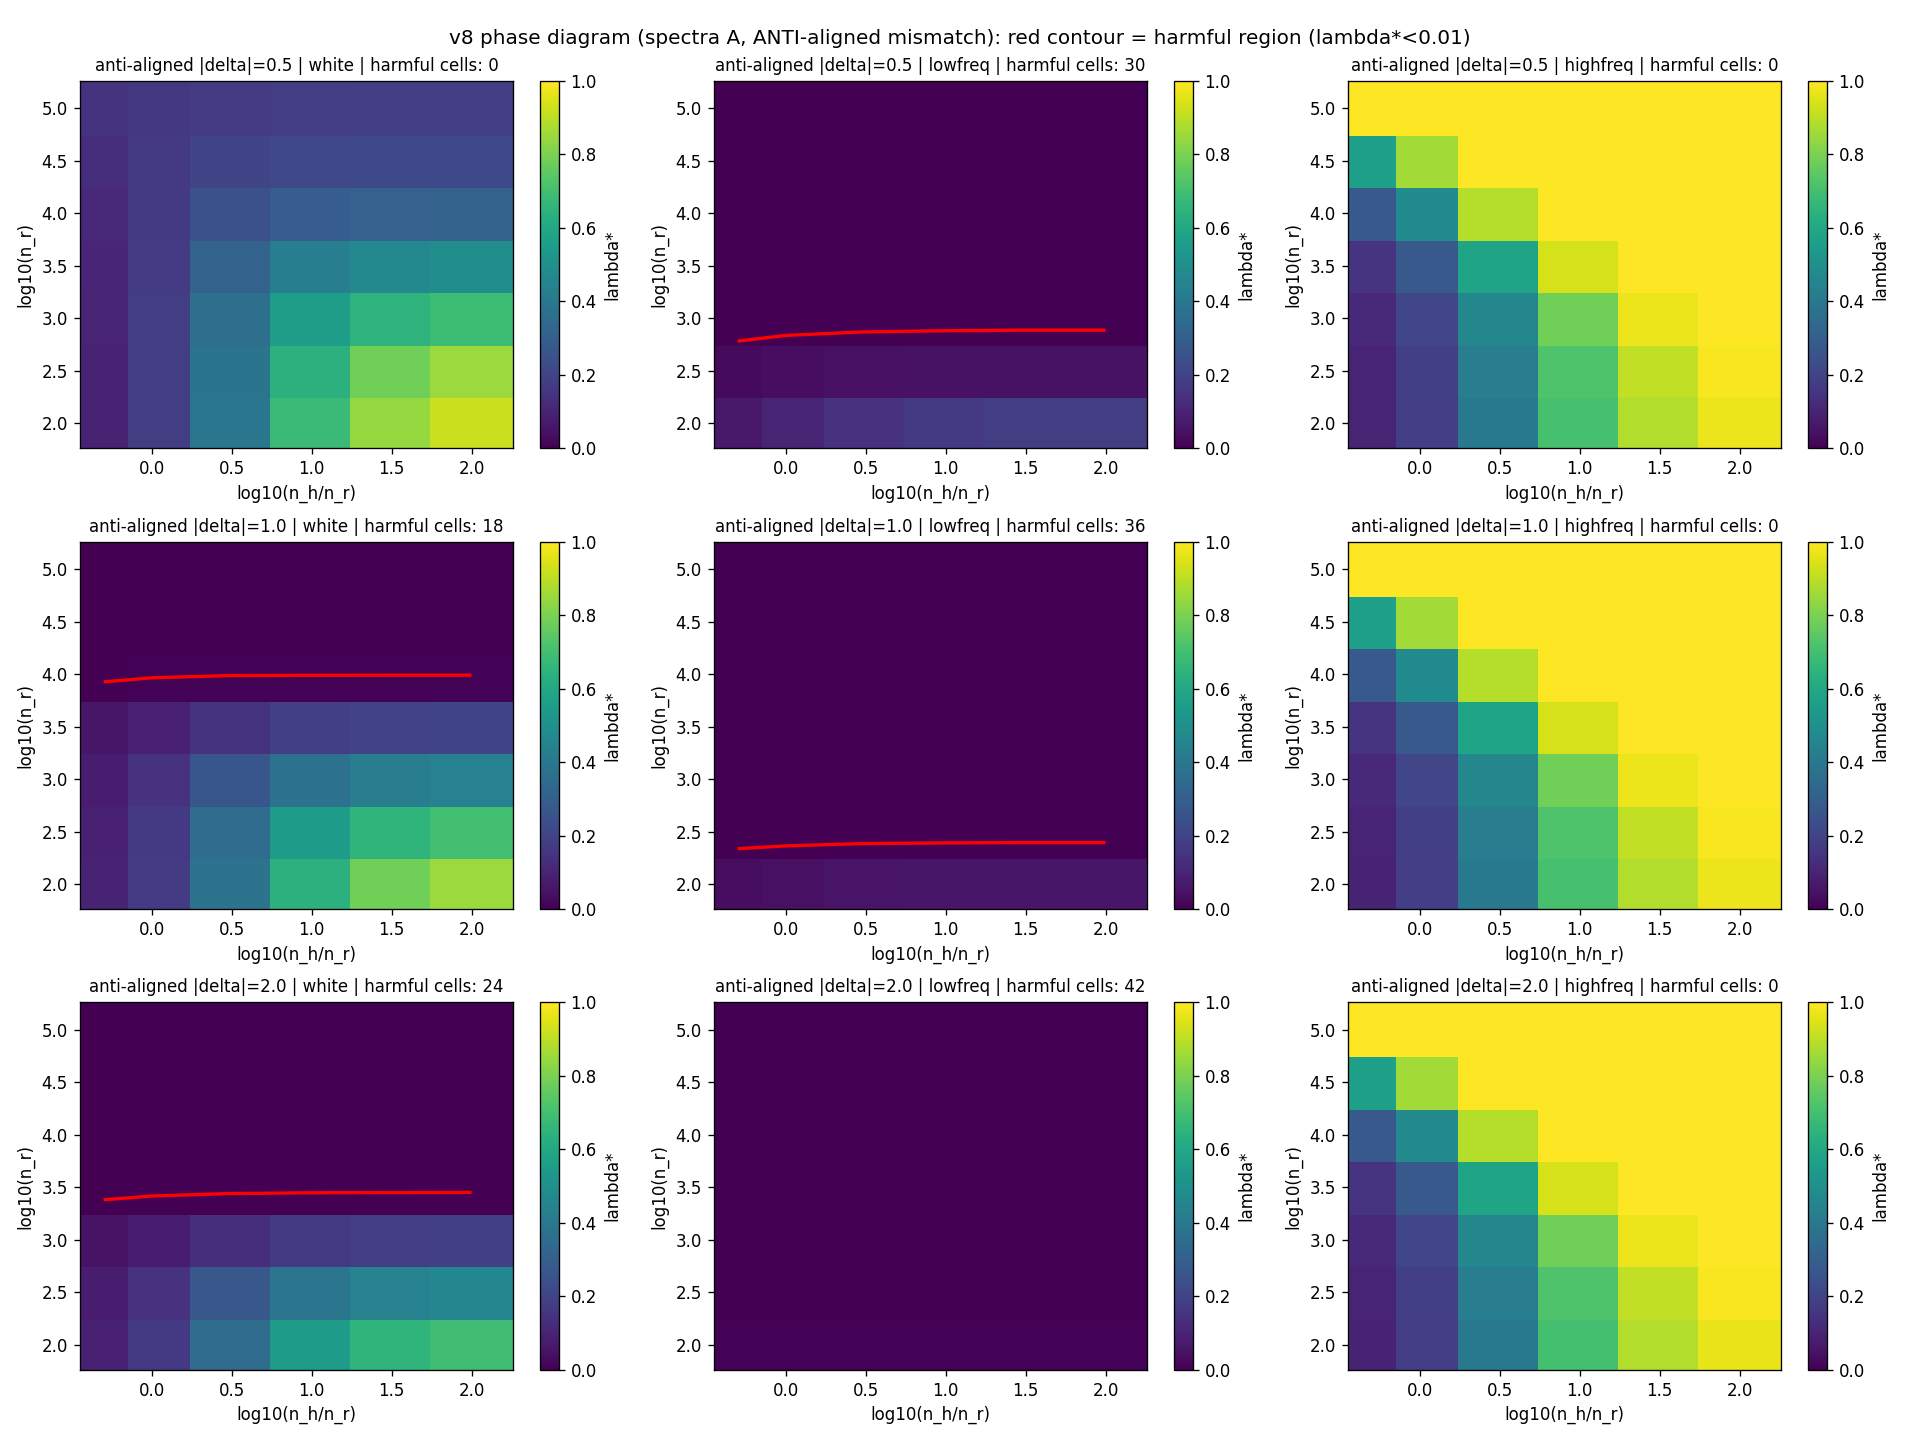
\includegraphics[width=\linewidth]{fig/phase_v8_anti.png}
  \caption{Optimal mixing ratio $\lambda^*$ over the $(\nr, \nh/\nr)$ plane under anti-aligned mismatch (spectral family A), by mismatch magnitude (rows) and spectral location (columns). Red contour: harmful region ($\lambda^*<0.01$).
  In this uncontrolled grid, low-frequency mismatch is harmful almost everywhere and high-frequency mismatch is harmless; location, target-weighted energy, and alignment vary together. The controlled candidate-family experiment in Sec.~\ref{supp:exp} finds no sign flip of $H$ after these invariants are fixed.}
  \label{supp:fig:phase}
\end{figure}

\textbf{(v12)} Exchange-rate numerics as in Sec.~\ref{supp:t2}.

\textbf{(v13) Unimodality verification.} Randomized checks of the results of Sec.~\ref{supp:t2} (\texttt{verify\_kex\_unimodality.py}): the affine derivative identity of Lemma~\ref{supp:lem:affine} matches finite differences to $7\times10^{-6}$ (the finite-difference accuracy) over $2\times10^5$ random draws; the forbidden sign pattern of Proposition~\ref{supp:prop:nomax} never occurs, and all $\sim10^5$ interior roots found are minima; the quadratic form of Theorem~\ref{supp:thm:quad} holds to $2\times10^{-14}$ with the closed-form $\lambda^*$ matching the numerical argmin; condition~\eqref{supp:eq:convreg} implies convexity in every one of the $1.8\times10^4$ draws in which it holds; and a targeted search over $4\times10^3$ aggregate risks (power-law and adversarial spectra) found no multimodal instance.

\textbf{(v14) Dosage law and closed-form $\kex$.} (\texttt{verify\_dosage\_law.py}.) Corollary~\ref{supp:cor:interior}: in $3.96\times10^4$ random general-spectrum draws with both endpoint signs strict, the global minimizer is interior in 100\% of cases. Theorem~\ref{supp:thm:dosage}: over 212 matched-spectrum configurations (8 decades of $\nh$ each), the closed-form gain, the closed-form $\kex$, and the $\nh^\varepsilon$ inversion match direct evaluation of the same leading-order per-coordinate risk (pointwise evaluation / bisection of the defining equation) to $3\times10^{-10}$, $1.1\times10^{-10}$, and $3\times10^{-16}$ respectively, and $\lambda^*(\nh)$ is nondecreasing in every tested configuration.

\textbf{(v16) Full-ridge numerical surrogate.} (\texttt{verify\_full\_ridge.py}.) Monte-Carlo risk of the full ridge estimator against $\mathrm{MSE}^{\mathrm{full,num}}$: relative errors between $-8.4\%$ and $+0.4\%$ across four configurations, decaying with sample size ($-2.5\% \to +0.3\%$ as $n_r$ grows $100 \to 6400$); on the same configurations the T1-a form overestimates by $+4\%$ to $+61\%$, consistent with the second-order feedthrough-recovery conjecture but not establishing a theorem-level upper bound; the mismatch sandwich converges to its per-coordinate price on these nondegenerate configurations (errors $-0.3\%$ to $+8\%$).

\section{A label-shift floor for aligned representations (boundary)}
\label{supp:zhao}

This section formalizes boundary (a) stated in the main text: when alignment is enforced on representations whose \emph{action marginals} differ, a shared deterministic head provably fails on the target domain.
It is the squared-loss, mixture-distribution analogue of the classical bound of Zhao et al.\ (cited in the main text).

Setup: a representation $z = \Phi(x)$ with induced feature laws $P_r^z, P_h^z$ satisfying $W_1(P_r^z, P_h^z) \le \varepsilon$; action marginals $P_e^a$ with means $\mu_e$, gap $\Delta\mu = \mu_h - \mu_r$; a deterministic $L$-Lipschitz head $f$; domain risks $R_e(f) = \E[(f(z) - y_e)^2]$.

\begin{proposition}[label-shift floor]\label{supp:prop:zhao}
For every deterministic head $f$:
\begin{enumerate}
\item[(i)] $R_r(f) + R_h(f) \ge \tfrac12\big(|\Delta\mu| - L\varepsilon\big)_+^2$;
\item[(ii)] the mixture risk $R_\lambda(f) = (1-\lambda)R_r(f) + \lambda R_h(f)$ obeys
\begin{equation}
R_\lambda(f) \ge \lambda(1-\lambda)\big(|\Delta\mu| - L\varepsilon\big)_+^2;
\end{equation}
\item[(iii)] any head with $R_\lambda(f) \le \eta$ pays target risk
$R_r(f) \ge \big(|\Delta\mu| - L\varepsilon - \sqrt{\eta/\lambda}\,\big)_+^2$. We do not assert a stronger floor for an unspecified mixture-optimal head.
\end{enumerate}
\end{proposition}

\begin{proof}
Write $\nu_e = \E_{z \sim P_e^z}[f(z)]$.
By Jensen, $R_e(f) \ge (\nu_e - \mu_e)^2$, and by the Kantorovich--Rubinstein dual, $|\nu_r - \nu_h| \le L\, W_1(P_r^z, P_h^z) \le L\varepsilon$.
(i)~$(\nu_r-\mu_r)^2 + (\nu_h-\mu_h)^2 \ge \tfrac12\big((\nu_r-\mu_r) - (\nu_h-\mu_h)\big)^2 \ge \tfrac12(|\Delta\mu| - L\varepsilon)_+^2$, since $(\nu_r-\mu_r) - (\nu_h-\mu_h) = -\Delta\mu + (\nu_r - \nu_h)$.
(ii)~Minimize $(1-\lambda)(\nu_r-\mu_r)^2 + \lambda(\nu_h-\mu_h)^2$ subject to $|\nu_r-\nu_h| \le L\varepsilon$. For fixed shift $\delta = \nu_h - \nu_r$, the minimum over the common level is attained at $\nu_r = (1-\lambda)\mu_r + \lambda(\mu_h - \delta)$ with value $\lambda(1-\lambda)(\Delta\mu - \delta)^2$; minimizing over $\delta \in [-L\varepsilon, L\varepsilon]$ gives $\delta^* = \mathrm{sign}(\Delta\mu)\min(L\varepsilon, |\Delta\mu|)$ and value $\lambda(1-\lambda)(|\Delta\mu| - L\varepsilon)_+^2$.
(iii)~$R_\lambda(f) \le \eta$ implies $|\nu_h - \mu_h| \le \sqrt{\eta/\lambda}$, hence $|\nu_r - \mu_r| \ge |\Delta\mu| - L\varepsilon - \sqrt{\eta/\lambda}$. Squaring and using $R_r(f) \ge (\nu_r - \mu_r)^2$ gives the displayed bound.
\end{proof}

\begin{remark}[Bernoulli case]
For binary actions $y \in \{0,1\}$, $|\Delta\mu| = D_{\mathrm{TV}}(P_r^a, P_h^a)$ and (i) is the Brier-score analogue of the classification bound of Zhao et al.: perfectly aligned representations with shifted label marginals are guaranteed to fail --- exact alignment ($\varepsilon \to 0$) does not remove the floor, it creates it.
For continuous actions the first-moment gap is the sharp quantity; second-moment (variance) shifts give analogous floors with second moments in place of means.
\end{remark}

\begin{remark}[operational reading for the L1 test]
The floor is monotone in the marginal gap and applies to any head whose mixture risk is already small. It provides a target-risk bound, not an identification of the actual mixture-optimal head or of its exact risk.
The quantitative prediction for the action-marginal-shift axis of the companion policy-level study is therefore stated only through the general low-mixture-risk bound, not through a separate $\lambda^2$ optimum formula.
Numerical checks (\texttt{verify\_zhao\_floor.py}): bounds (i)--(iii) hold on $2\times10^5$ random draws with zero violations; the mean-level constrained quadratic solution matches brute-force minimization. These checks do not identify an optimal head in the original function class.
\end{remark}

\section{Theorem T1-b: a full-ridge population equivalent (fixed-$p$ regime)}
\label{supp:t1b}

We prove a leading-order result for the fixed-dimension regime and explicitly separate it from second-order numerical corrections.
The full ridge estimator is $\hat\beta = A^{-1}(w_r X_r^\top y_r + w_h X_h^\top y_h)$ with $A = w_r S_r + w_h S_h + \mu I$ and $S_e = X_e^\top X_e$ the (non-diagonal) sample Gram matrices, in the model of Sec.~\ref{supp:setup}.
Define
\begin{align}
  \riske^{\mathrm{full}}(\lambda)
  &:= \sum_j \frac{a_j}{D_j^2}\Big[V_j(\lambda)+(\lambda b_j\delta_j-\mu\beta^*_j)^2\Big], \notag\\
  V_j(\lambda)&=\frac{(1-\lambda)^2\sigma_r^2a_j}{\nr}+\frac{\lambda^2\sigma_h^2b_j}{\nh}.
  \label{supp:eq:t1b-pop}
\end{align}

\begin{theorem}[T1-b: population-level approximation]\label{supp:thm:t1b}
Let the covariates be Gaussian, $p$ fixed, $\mu > 0$ fixed, and $\nr, \nh \to \infty$ at fixed $\lambda \in (0,1)$.
Then
\begin{equation}
  \big|\risk(\lambda)-\riske^{\mathrm{full}}(\lambda)\big| = O(n^{-1/2}),
  \qquad n=\min(\nr,\nh),
  \label{supp:eq:t1b}
\end{equation}
where the constants depend on $(p,\mu^{-1},\|\beta^*\|,\|\delta\|)$ and the spectra.
In words: the population full-ridge risk is the T1-a leading form with the feedthrough-corrected noise $\tilde\sigma_e^2=\sigma_e^2+F_e$ replaced by the true label noise $\sigma_e^2$.
This theorem does \emph{not} control $O(1/n)$ terms, derivatives with respect to $\lambda$, or errors of optimized risks.
\end{theorem}

\begin{proof}
The error decomposes exactly as
\begin{equation}
\begin{gathered}
\hat\beta - \beta^* = -\mu A^{-1}\beta^* + A^{-1} w_h S_h\, \delta + A^{-1}\eta,
\\[2pt]
\eta = w_r X_r^\top\varepsilon_r + w_h X_h^\top\varepsilon_h .
\end{gathered}
\end{equation}
Two estimates drive everything: (1)~Wishart concentration, $\|S_e/n_e - \Sigma_e\| = O_p(\sqrt{p/n_e})$, hence $\|A - D\| = O_p(n^{-1/2})$ with $D = (1-\lambda)\Sigma_r + \lambda\Sigma_h + \mu I = \mathrm{diag}(D_j)$; (2)~resolvent perturbation, using the deterministic bound $\|A^{-1}\| \le 1/\mu$: on the event $\|A-D\| \le \mu/2$ (whose complement is exponentially unlikely),
\begin{equation}
\|A^{-1} - D^{-1}\| \;\le\; \|A-D\|\,\big/\,\big(\mu\,(\mu-\|A-D\|)\big) \;=\; O_p(n^{-1/2}) .
\end{equation}
For the mismatch term write $w_h S_h\delta = \lambda\Sigma_h\delta + \zeta$ with $\E\|\zeta\|^2 = (\lambda^2/\nh)\,\mathrm{Var}\big(x(x^\top\delta)\big) = O(1/\nh)$; hence the mismatch-plus-shrinkage risk converges to $\sum_j a_j(\lambda b_j\delta_j - \mu\beta^*_j)^2/D_j^2$, including the alignment cross term.
For the variance, $\E[\eta\eta^\top \mid X] = w_r^2\sigma_r^2 S_r + w_h^2\sigma_h^2 S_h$, so $\E[\eta^\top A^{-1}\Sigma_r A^{-1}\eta]$ converges to $\mathrm{tr}\, \Sigma_r D^{-1}\big((1-\lambda)^2\sigma_r^2\Sigma_r/\nr + \lambda^2\sigma_h^2\Sigma_h/\nh\big)D^{-1}$, the displayed variance sum.
Cross terms involving $\eta$ vanish by conditional centering, and all replacements of $A^{-1}$ by $D^{-1}$ are justified by the deterministic bound $\|\Sigma_r^{1/2}A^{-1}\Sigma_e^{1/2}\| \le (\max_j a_j \cdot \max_j \lambda^e_j)^{1/2}/\mu^2$ on the good event.
The complementary event is exponentially unlikely and the relevant estimators have finite fourth moments, so the stated order also holds for the expected risk $\risk$; the remainder is not a stochastic symbol attached to an already-averaged object.
\end{proof}

\paragraph{Why population accuracy is not second-order accuracy.}
Take $p=1$, $a=b=\beta^*=1$, $\lambda=1/2$, $\delta=0.2$, $\mu=0.1$, $\nr=\nh=1000$, and zero label noise.
Then $\lambda b\delta-\mu\beta^*=0$ and $D=1.1$, so Eq.~\eqref{supp:eq:t1b-pop} gives zero risk.
The actual estimator nevertheless has positive risk from sample-Gram fluctuations: an independent $2\times10^6$-replicate calculation gives $1.6542\times10^{-5}$ (standard error $1.66\times10^{-8}$), while the first nonzero fluctuation term is
\begin{equation}
  \frac{2\lambda^2(b\delta)^2/\nh}{D^2}=1.65289\times10^{-5}.
  \label{supp:eq:t1b-cancellation}
\end{equation}
This is fully compatible with the $O(n^{-1/2})$ remainder, but demonstrates that the theorem cannot justify $O(1/n)$ coefficients or exact cancellation claims.

\paragraph{A legacy numerical surrogate, distinct from the proved T1-c object.}
Our earlier full-ridge numerical curves use $\mathrm{MSE}^{\mathrm{full,num}}$: Eq.~\eqref{supp:eq:t1b-pop} with the mismatch-fluctuation term $2\lambda^2(b_j\delta_j)^2/(\nh D_j^2)$ and the same denominator corrections $-4N_{0j}\mathrm{Cov}(\tilde n_j,\hat D_j)/D_j^3+3N_{0j}^2\mathrm{Var}(\hat D_j)/D_j^4$ as in the diagonal analysis (\texttt{mse\_t1b} in the code).
This is a computational surrogate motivated by the diagonal expansion; it is not the second-order object proved in T1-c below.
In the cancellation example above, the surrogate gives exactly Eq.~\eqref{supp:eq:t1b-cancellation}, whereas the population display gives zero.

\paragraph{Consequences and non-consequences.}
(i)~\emph{Mismatch sandwich at a nondegenerate scale.}
Write $\mathcal B_{\mathrm{mis}}^0=\sum_j a_j(\lambda b_j\delta_j/D_j)^2$.
The same resolvent estimates give $\mathcal B_{\mathrm{mis}}=\mathcal B_{\mathrm{mis}}^0(1+o(1))$ when $\mathcal B_{\mathrm{mis}}^0$ dominates the $n^{-1/2}$ remainder scale.
No relative-error claim is made when $\mathcal B_{\mathrm{mis}}^0=0$ or is itself $O(1/n)$.

(ii)~\emph{Feedthrough recovery is a second-order conjecture with numerical support, not a consequence of T1-b.}
The proposed difference $\sum_j a_j[(1-\lambda)^2F_raj/\nr+\lambda^2F_hb_j/\nh]/D_j^2$ is $O(1/n)$, smaller than the theorem's remainder.
Thus T1-b cannot establish its sign or magnitude, and we do not claim a theorem-level variance upper bound for T1-a; the v6/v16 results are numerical evidence only.

(iii)~\emph{No blanket downstream transfer.}
Corollary~1, Theorem~2, Corollary~2, and the dosage law involve derivatives, $O(1/n)$ coefficients, or optimized risks.
They therefore do not follow from T1-b by substituting $\tilde\sigma_e^2\to\sigma_e^2$.
The complete fixed-$p$ second-order risk and zero-mixing derivative are proved separately below. Uniform derivatives and optimized-risk control are established only for a unique, nondegenerate interior population optimum; boundary-switching and general downstream transfer remain open.

\subsection{Complete second-order risk at fixed dimension}

\begin{theorem}[T1-c: full-ridge second-order risk]\label{supp:thm:t1c}
Under the Gaussian fixed-$p$ assumptions of Theorem~\ref{supp:thm:t1b}, let $\rho=\nh/\nr$ be fixed. Then, uniformly for $\lambda\in[0,1]$,
\begin{equation}
 R_{\mathrm{full}}(\lambda;\nr)=R_0(\lambda)+\frac{R_1(\lambda)}{\nr}+o(\nr^{-1}).
 \label{supp:eq:t1c}
\end{equation}
Define $D=(1-\lambda)\Sigma_r+\lambda\Sigma_h+\mu I$, $R=D^{-1}$, $S=R\Sigma_rR$, $v=-\mu\beta^*+\lambda\Sigma_h\delta$, and
\begin{align}
 \mathcal T_e(N)&=\Sigma_eN\Sigma_e+\operatorname{tr}(\Sigma_eN)\Sigma_e,\notag\\
 \mathcal T&=(1-\lambda)^2\mathcal T_r+\lambda^2\rho^{-1}\mathcal T_h,\notag\\
 U&=\mathcal T(R),\notag\\
 C&=RUS+SUR+R\mathcal T(S)R.
 \label{supp:eq:t1c-matrices}
\end{align}
The coefficients are $R_0=v^\top Sv$ and
\begin{align}
 R_1={}&v^\top Cv+\frac{\lambda^2}{\rho}\operatorname{tr}\{S\mathcal T_h(\delta\delta^\top)\}\notag\\
 &-\frac{2\lambda^2}{\rho}v^\top[R\mathcal T_h(S)+S\mathcal T_h(R)]\delta\notag\\
 &+(1-\lambda)^2\sigma_r^2\operatorname{tr}(S\Sigma_r)
 +\frac{\lambda^2\sigma_h^2}{\rho}\operatorname{tr}(S\Sigma_h).
 \label{supp:eq:t1c-r1}
\end{align}
This is a risk expansion, not yet a uniform derivative or optimized-risk theorem.
\end{theorem}

\begin{proof}[Proof sketch]
Write $G_e=X_e^\top X_e/n_e$, $Z_e=G_e-\Sigma_e$, $B=[(1-\lambda)G_r+\lambda G_h+\mu I]^{-1}$, and $Z=(1-\lambda)Z_r+\lambda Z_h$. Conditional on both designs, the label-noise covariance is
$N=(1-\lambda)^2\sigma_r^2G_r/\nr+\lambda^2\sigma_h^2G_h/\nh$.
The exact risk is
\begin{equation}
 \mathbb E[(v+\lambda Z_h\delta)^\top B\Sigma_rB(v+\lambda Z_h\delta)]
 +\mathbb E\operatorname{tr}\{\Sigma_rBNB\}.
 \label{supp:eq:t1c-exact}
\end{equation}
The real Wishart moment is $\mathbb E[Z_eNZ_e]=\mathcal T_e(N)/n_e$, so $\mathbb E[ZNZ]=\mathcal T(N)/\nr$. On $\|Z\|\le\mu/2$, use $B=R-RZR+RZRZR+O_p(\|Z\|^3)$. Pairing the two fluctuations gives $\mathbb E[B\Sigma_rB]=S+C/\nr+o(\nr^{-1})$.
The mismatch square contributes the second term of Eq.~\eqref{supp:eq:t1c-r1}. Although $\mathbb EZ_h=0$, its cross term with $B$ is of order $\nr^{-1}$ and gives the third term. The label-noise term gives the final two terms; its further resolvent corrections are $O(\nr^{-2})$.
The good-event remainder is $O_p(\nr^{-3/2})$. On the exponentially unlikely complementary event, both the actual-risk contribution and the subtracted deterministic approximation are controlled using $\|B\|\le\mu^{-1}$, finite fourth moments, and Cauchy--Schwarz. The same good event and continuous coefficients give uniformity in $\lambda\in[0,1]$, including the endpoints.
\end{proof}

\paragraph{Numerical verification of T1-c.}
The script \texttt{verify\_full\_ridge\_second\_order.py} checks 22 design-level conditional-risk cells over $p=1,2,20$, aligned and anti-aligned mismatch, $\lambda\in\{0,0.1,0.3,0.5,0.8,1\}$, and $\nr=1000,4000$. All simulated means are within $2.13$ Monte-Carlo standard errors of Eq.~\eqref{supp:eq:t1c}; three direct actual-estimator checks are within $1.12$ standard errors. Compact-versus-pairwise algebra and consistency with the zero-mixing derivative have maximum error $7.11\times10^{-15}$. The one-dimensional cancellation example recovers the first positive risk term. The legacy surrogate is compared separately in \texttt{compare\_full\_ridge\_surrogate.py}; it is not the object proved here.

\subsection{The standard full-ridge zero-mixing derivative}

\begin{theorem}[Fixed-$p$ derivative with the first Gram correction]\label{supp:thm:fullprime}
Under the Gaussian fixed-$p$ assumptions of Theorem~\ref{supp:thm:t1b}, the actual full-ridge target risk satisfies
\begin{equation}
  R_{\mathrm{full}}'(0^+;\nr)=H_{\mathrm{full}}-\frac{K_{\mathrm{full}}}{\nr}+o(\nr^{-1}).
  \label{supp:eq:fullprime}
\end{equation}
The limit in the shared spectral basis is
\begin{equation}
 H_{\mathrm{full}}=-2\mu\sum_j\frac{a_jb_j\beta_j^*\delta_j}{(a_j+\mu)^2}
 -2\mu^2\sum_j\frac{a_j\beta_j^{*2}(b_j-a_j)}{(a_j+\mu)^3},
\end{equation}
but $K_{\mathrm{full}}$ is not obtained by differentiating the population risk alone.
Write $\Sigma=\Sigma_r$, $D_0=\Sigma+\mu I$, $R=D_0^{-1}$, $S=R\Sigma R$, $M=\Sigma_h-\Sigma$, and
\begin{equation}
  \mathcal T(N)=\Sigma N\Sigma+\operatorname{tr}(\Sigma N)\Sigma,\qquad U=\mathcal T(R).
\end{equation}
Define the coefficient matrices
\begin{align}
  \mathcal C={}&RUS+SUR+R\mathcal T(S)R,\notag\\
  \mathcal L={}&\mathcal J(M)+R\mathcal T(S)R+2SUR,\notag\\
  \mathcal J(N)={}&RUSNR+SURNR+SNRUR\notag\\
  &+R\mathcal T(S)RNR+R\mathcal T(SNR)R+S\mathcal T(RNR)R.
  \label{supp:eq:fullgram}
\end{align}
Then
\begin{align}
  K_{\mathrm{full}}={}&K_0-H_1,\qquad
  K_0=2\sigma_r^2\operatorname{tr}\{\Sigma(R\Sigma R+R\Sigma RMR)\},\notag\\
  H_1={}&-2\mu(\Sigma_h\delta)^\top\mathcal C\beta^*
  -2\mu^2\beta^{*\top}\mathcal L\beta^*.
  \label{supp:eq:kfull}
\end{align}
The expansion is uniform in a sufficiently small interval $\lambda\in[0,\varepsilon]$.
\end{theorem}

\begin{proof}[Proof sketch]
Let $G=X_r^\top X_r/\nr$, $B=(G+\mu I)^{-1}$, and $Z=G-\Sigma$. Differentiating the exact error decomposition, averaging over the independent human design and label noise, and using $\mathbb E[\eta_0\eta_0^\top\mid X_r]=\sigma_r^2G/\nr$ gives
\begin{align}
  R_{\mathrm{full}}'(0^+)={}&-2\mu(\Sigma_h\delta)^\top\mathbb E[B\Sigma B]\beta^*\notag\\
  &-2\mu^2\beta^{*\top}\mathbb E[B\Sigma B(\Sigma_h-G)B]\beta^*\notag\\
  &-\frac{2\sigma_r^2}{\nr}\operatorname{tr}\Sigma\,\mathbb E[BGB]\notag\\
  &-\frac{2\sigma_r^2}{\nr}\operatorname{tr}\Sigma\,\mathbb E[B(\Sigma_h-G)BGB].
  \label{supp:eq:fullexactprime}
\end{align}
For deterministic $N$, the real Wishart moment is
$\mathbb E[ZNZ]=\mathcal T(N)/\nr$. On the event $\|Z\|\le\mu/2$, expand
$B=R-RZR+RZRZR+O_p(\|Z\|^3)$.
Pairing the two $Z$ factors yields
\begin{align}
  \mathbb E[B\Sigma B]&=S+\mathcal C/\nr+o(\nr^{-1}),\notag\\
  \mathbb E[B\Sigma B(\Sigma_h-G)B]&=SMR+\mathcal L/\nr+o(\nr^{-1}).
\end{align}
The last two terms in Eq.~\eqref{supp:eq:fullexactprime} contribute $-K_0/\nr+O(\nr^{-2})$; collecting the bias correction $H_1/\nr$ proves Eq.~\eqref{supp:eq:kfull}. The complementary event is exponentially unlikely at fixed $p$, while $\|A^{-1}\|\le\mu^{-1}$ and the finite-moment assumptions control its contribution. The same bounds permit differentiation under the expectation and are uniform near $\lambda=0$.
\end{proof}

\begin{remark}[Identifiability and the critical-size interpretation]
Set $t=1/\nr$ and $\bar g(t)=H_{\mathrm{full}}-K_{\mathrm{full}}t$. A positive asymptotic critical scale
$\nr^{\mathrm{crit,full}}=K_{\mathrm{full}}/H_{\mathrm{full}}$
requires $H_{\mathrm{full}}K_{\mathrm{full}}>0$, and then $\bar g'(t^*)=-K_{\mathrm{full}}\ne0$. The sign is identifiable away from the root at any fixed relative distance. At the root itself the leading term vanishes and the remainder is still $o(\nr^{-1})$, so this is not an exact finite-sample root theorem. In particular, if $H_{\mathrm{full}}>0$ but $K_{\mathrm{full}}\le0$, no positive critical size follows from this expansion. This result does not transfer the dosage law, exchange rate, or global optimum.
\end{remark}

\paragraph{Numerical verification of the full-ridge derivative.}
The script \texttt{verify\_full\_ridge\_zero\_derivative.py} checks the compact matrices against an independent pairwise resolvent expansion (maximum discrepancy $1.11\times10^{-16}$) and against exact design-level conditional derivatives generated by Bartlett Wishart sampling. Across $p=1,2,20$ and $\nr=1000$--$16000$, all six Monte-Carlo cells agree with the prediction within sampling and higher-order error. For spectral family A at $p=20$, $\nr=1000$ gives prediction $0.0148136$ and Monte Carlo $0.0147617\pm0.0000197$; at $\nr=16000$ the values are $0.0263331$ and $0.0263323\pm0.0000052$. Direct actual-estimator finite differences at $\lambda=10^{-4}$ give $0.0143334\pm0.0003422$ for the former cell. These checks concern the zero-mixing derivative, not the general-$\lambda$ numerical surrogate.

\begin{remark}[the proportional regime]
For $p \asymp n$ the resolvent perturbation step fails and an anisotropic deterministic equivalent is needed.
The structure of a prospective proof is visible in the leave-one-out expansion of the sandwich: writing $S_h = \sum_i x_i x_i^\top$, the cross pairs $i \neq k$ carry the leading order through $\E[x\,(x^\top\delta)] = \Sigma_h\delta \neq 0$, while the diagonal pairs $i = k$ contribute only $O(1/\nh)$ corrections; a proportional-regime proof must therefore control $\sum_{i \neq k} (\delta^\top x_i)(x_i^\top A^{-1}\Sigma_r A^{-1} x_k)(\delta^\top x_k)$ via leave-two-out resolvent expansions --- the route through Wu's pipeline flagged in the project notes.
The fixed-$p$ second-order expansion and the nondegenerate interior-optimum theorem below do not extend to this regime; boundary-switching and general global-shape control also remain separate tasks.
\end{remark}

\section{Uniform derivatives and nondegenerate interior optima}
\label{supp:optfull}

\begin{theorem}[Uniform risk derivatives]\label{supp:thm:derivatives}
Under the fixed-$p$ assumptions of Theorem~\ref{supp:thm:t1c}, for $k=0,1,2$ and uniformly for $\lambda\in[0,1]$,
\begin{equation}
 R_{\mathrm{full}}^{(k)}(\lambda;\nr)
 =R_0^{(k)}(\lambda)+R_1^{(k)}(\lambda)/\nr+o(\nr^{-1}).
\end{equation}
Endpoints use one-sided derivatives.
\end{theorem}

\begin{proof}[Proof sketch]
The case $k=0$ is T1-c. On its uniform good event, bounded Gram norms and continuity give a fixed complex neighborhood of $[0,1]$ on which the empirical and population resolvents are analytic and uniformly bounded. The conditional risk and the coefficients $R_0,R_1$ are therefore analytic there. Apply Cauchy's integral formula to the analytic risk remainder on a fixed contour; the uniform $o(\nr^{-1})$ risk remainder implies the same order for its first two derivatives. On the exponentially unlikely complementary event, the actual derivative and the subtracted deterministic derivative are separately controlled by the resolvent bound and finite-moment assumptions.
\end{proof}

\begin{theorem}[Nondegenerate interior optimum]\label{supp:thm:optfull}
Suppose $R_0$ has a unique global minimizer $w_0\in(0,1)$ with $R_0''(w_0)>0$. Write $R_n(w)=R_{\mathrm{full}}(w;\nr)$. For all sufficiently large $\nr$, $R_n$ has a unique global minimizer $w_n^*$ on $[0,1]$, and
\begin{align}
 w_n^*&=w_0-\frac{R_1'(w_0)}{\nr R_0''(w_0)}+o(\nr^{-1}),\notag\\
 R_n(w_n^*)&=R_0(w_0)+R_1(w_0)/\nr+o(\nr^{-1}),\\
 \mathcal G_n:=R_n(0)-R_n(w_n^*)&=\mathcal G_0+\mathcal G_1/\nr+o(\nr^{-1}),\notag
\end{align}
where $\mathcal G_0=R_0(0)-R_0(w_0)$ and $\mathcal G_1=R_1(0)-R_1(w_0)$. When $R_1'(w_0)=0$, the display gives $\nr(w_n^*-w_0)\to0$; the direction of the shift is then determined only at higher order.
\end{theorem}

\begin{proof}
Choose a neighborhood $I_\delta$ of $w_0$ on which $R_0''>0$. Uniform second-derivative control makes $R_n$ strictly convex there. Outside $I_\delta$, the unique population minimizer leaves a positive risk gap, and uniform risk control excludes a global minimizer. The signs of $R_n'$ at the two endpoints of $I_\delta$ follow from uniform first-derivative control, so the unique interior convex minimizer is global. Since $\delta$ is arbitrary, $w_n^*\to w_0$. The optimized-risk display then follows by continuity and the uniform risk expansion.

It remains to prove the weight rate. Put $c=R_0''(w_0)>0$, $d=R_1'(w_0)$, and $A_*=-d/c$. The explicit matrix coefficients in Theorem~\ref{supp:thm:t1c} are analytic in a fixed neighborhood of $w_0$. For every fixed $A$, the uniform first-derivative expansion evaluated at $w_0+A/\nr$, Taylor's theorem applied to $R_0'$, and continuity of $R_1'$ give
\begin{align}
 \nr R_n'(w_0+A/\nr)
 &=\nr R_0'(w_0+A/\nr)+R_1'(w_0+A/\nr)+o(1)\notag\\
 &=cA+d+o(1).
 \label{supp:eq:scaled-optimal-derivative}
\end{align}
For any $A_-<A_*<A_+$, the limits $cA_-+d<0$ and $cA_++d>0$ imply that, for all sufficiently large $\nr$, $R_n'$ is negative at $w_0+A_-/\nr$ and positive at $w_0+A_+/\nr$. These points eventually lie in $I_\delta$, where $R_n$ is strictly convex, so the stationary point between them is the unique global minimizer $w_n^*$. Choosing $A_-=A_*-\varepsilon$ and $A_+=A_*+\varepsilon$ for arbitrary $\varepsilon>0$ proves $\nr(w_n^*-w_0)\to A_*$, as claimed.
\end{proof}

\begin{theorem}[Nondegenerate and flat left-boundary optima]\label{supp:thm:boundaryfull}
Suppose $w=0$ is the unique global minimizer of $R_0$ on $[0,1]$. If $R_0'(0^+)>0$, then $w_n^*=0$ for all sufficiently large $\nr$. If instead $R_0'(0^+)=0$ and $c=R_0''(0^+)>0$, then the sign of $d=R_1'(0^+)$ determines the direction: $d>0$ gives $w_n^*=0$ for all sufficiently large $\nr$, while $d<0$ gives
\begin{equation}
 w_n^*\sim-d/(c\nr),\qquad \mathcal G_n\sim d^2/(2c\nr^2).
\end{equation}
The case $d=0$ is undetermined at this order. The right boundary is analogous when $R_0'(1^-)<0$.
\end{theorem}

\begin{proof}[Proof sketch]
In the nondegenerate case, uniform first-derivative control preserves strict increase near zero, while the population risk gap and uniform risk control exclude all other global minimizers. In the flat case, $d>0$ gives the same boundary conclusion. For $d<0$, evaluating $R_n'(A/\nr)=(cA-d+o(1))/\nr$ on both sides of $A=|d|/c$ proves $\nr w_n^*\to|d|/c$. For the gain, integrate the derivative expansion rather than subtracting the $o(\nr^{-1})$ risk remainders:
$\mathcal G_n=-\int_0^{w_n^*}R_n'(w)\,dw$. The integral has the required $o(\nr^{-2})$ remainder and yields $\mathcal G_n\sim d^2/(2c\nr^2)$.
\end{proof}

\paragraph{A local-harm/global-benefit counterexample.}
The script \texttt{verify\_full\_ridge\_counterexample.py} verifies a three-dimensional configuration with $R_0'(0^+)=0.2628138>0$ but an interior global minimizer $w_0=0.0682897$ satisfying $R_0(0)=0.0338052$ and $R_0(w_0)=0.0247415$, with $R_0''(w_0)=3.44659$. At $\nr=1000$, the actual zero-mixing derivative is $0.221174$ (prediction $0.221356$), while the optimized gain is $0.009396$ (prediction $0.009405$). Hence $R_0'(0^+)>0$ alone cannot imply global discard; the global-minimum-at-zero shape condition in Theorem~\ref{supp:thm:boundaryfull} is essential. Boundary scaling checks use \texttt{verify\_full\_ridge\_boundary.py}, including a high-replication flat-boundary cell.

\paragraph{Numerical verification.}
The script \texttt{verify\_full\_ridge\_global\_optimum.py} checks 16 design-level derivative cells and two paired actual-estimator center differences, followed by nondegenerate optima in the one-dimensional cancellation example and a two-dimensional aligned example. Direct derivative checks are within $0.73$ standard errors; four optimized-risk checks are within $1.59$ standard errors. In the latter example, $w_0=0.3708597$ and $R_0''(w_0)=0.13996$; at $\nr=1000,4000$, the predicted optimized risks are $0.01063196$ and $0.01002290$, compared with Monte Carlo $0.01063452$ and $0.01002470$.

The separate script \texttt{verify\_full\_ridge\_weight\_expansion.py} checks the new weight rate by fitting roots of average conditional-derivative curves, rather than averaging per-replicate argminima. In the two-dimensional example, $R_1'(w_0)=0.320971$ and the limiting scaled shift is $-2.29329$. The optima of the first-order coefficient curve have scaled shifts $-2.07343,-2.17785,-2.23408,-2.26330$ at $\nr=500,1000,2000,4000$, approaching this limit. The $\nr=500$ cell has visible higher-order deviation and is not counted as an asymptotic fit success. At $\nr=4000$, 200{,}000 conditional-design replicates give a Monte Carlo scaled shift of $-2.29688\pm0.07803$. In the near-zero cancellation example, the predicted constant is $-0.09091$; all eight 20{,}000-replicate root estimates are within $1.98$ Monte Carlo standard errors, although these intervals are comparatively wide. Independent actual-E2 paired derivative checks at $\nr=1000$ give $-0.000435\pm0.000137$ and $0.000469\pm0.000137$ on the left and right of the first-order weight prediction, with the expected signs. These checks do not address boundary-switching or flat/multiple optima.

\section{Matched-spectrum full-ridge gain, exchange approximation, and surrogate dosage}
\label{supp:doseexchange}

For matched spectra, $R_0(w)=A_0+A_1w+A_2w^2$ with $A_2$ independent of $\rho=\nh/\nr$, and $R_1(w;\rho)=C_0(w)+C_1(w)/\rho$. If $A_2>0$, the population optimum is $w_0=\operatorname{clip}_{[0,1]}(-A_1/(2A_2))$, with
\begin{equation}
 G_0=\begin{cases}
 0,&A_1\ge0,\\
 A_1^2/(4A_2),&A_1<0,\;-A_1<2A_2,\\
 -A_1-A_2,&A_1<0,\;-A_1\ge2A_2.
 \end{cases}
\end{equation}
Under the nondegenerate optimal-branch assumptions, $\mathcal G_n=G_0+G_1(\rho)/\nr+o(\nr^{-1})$, where $G_1=R_1(0)-R_1(w_0)=D_0+D_1/\rho$. Equivalently, $\mathcal G_n=G_0+D_0/\nr+D_1/\nh+o(\nr^{-1})$; this is a fixed-$\rho$ expansion, not a claim of uniformity as $\rho\to0$ or $\infty$.

\paragraph{Exact dosage rule for a quadratic surrogate.}
Write $S=R\Sigma R$, $C_r=\sigma_r^2\operatorname{tr}(S\Sigma)$, and $C_h=\sigma_h^2\operatorname{tr}(S\Sigma)$. Retaining population label noise defines the quadratic surrogate
$\widetilde R_{\nr,\nh}(w)=R_0(w)+C_r(1-w)^2/\nr+C_hw^2/\nh$, with
\begin{align}
 A_1^{\mathrm{lead}}&=A_1-2C_r/\nr,\notag\\
 A_2^{\mathrm{lead}}(\nh)&=A_2^r+B/\nh,\notag\\
 A_2^r&=A_2+C_r/\nr,\qquad B=C_h.
\end{align}
This surrogate omits sample-Gram fluctuation corrections that can be of order $\nr^{-1}$, the same order as its retained noise terms. Its dosage identity is therefore not a complete first-order full-ridge dosage expansion. For $A_2^{\mathrm{lead}}>0$, a nonnegative $A_1^{\mathrm{lead}}$ gives zero optimal gain at $w=0$. When $A_1^{\mathrm{lead}}<0$, the hyperbolic gain $(A_1^{\mathrm{lead}})^2/(4A_2^{\mathrm{lead}})$ applies only when $-A_1^{\mathrm{lead}}<2A_2^{\mathrm{lead}}(\nh)$; otherwise the boundary gain is $-A_1^{\mathrm{lead}}-A_2^{\mathrm{lead}}(\nh)$. If $-A_1^{\mathrm{lead}}>2A_2^r$, the boundary is reached at $\nh^b=B/(-A_1^{\mathrm{lead}}/2-A_2^r)$, and the boundary saturation value is $-A_1^{\mathrm{lead}}-A_2^r$ rather than the interior hyperbolic limit.

\paragraph{First-order exchange approximation and its pole.}
The target-only risk is $S+B_0/m+o(m^{-1})$, with $S=R_0(0)$ and $B_0=R_1(0)$, while the optimized mixture risk is $S-G_0+(B_0-G_1)/\nr+o(\nr^{-1})$. Assume $B_0>0$ and define $\Gamma_n^{(1)}=\nr G_0+G_1$. Dropping the remainders gives the approximate exchange equation
$B_0[1/\nr-1/(\nr+\kappa\nh)]=\Gamma_n^{(1)}/\nr$.
For $0<\Gamma_n^{(1)}<B_0$, its finite positive solution is
\begin{equation}
 \kex^{(1)}=\frac{\Gamma_n^{(1)}}{\rho(B_0-\Gamma_n^{(1)})}.
\end{equation}
When $\Gamma_n^{(1)}=0$, the solution is zero; for $\Gamma_n^{(1)}\ge B_0$, the approximate equation has no finite solution. If $G_0>0$, the pole is eventually crossed at fixed $\rho$. These are algebraic statements about the first-order equation and the fixed-$\mu$ baseline. They do not classify the actual finite-sample exchange rate near the pole, where discarded terms may change the sign. No uniform exchange error bound or unrestricted source-size dosage guarantee is claimed.

\paragraph{Numerical verification.}
The script \texttt{verify\_full\_ridge\_dosage\_exchange.py} compares the closed-form optimum with grid minimization of the same quadratic surrogate in 16 dose cells, with maximum gain discrepancy $1.49\times10^{-10}$, including a surrogate boundary crossing at $\nh=1779.1732$. This is an algebraic implementation check. Separately, for one full-ridge interior configuration, $G_1(\rho)=0.99757865-1.203415/\rho$; at $\nr=1000,\rho=6$, the predicted gain is $0.0122185831$ and 50{,}000 conditional-risk replicates give $0.0122262407\pm0.0000066100$. The first-order exchange equation has no finite solution for the same configuration at $\nr=1000$ in the tested ratios, while an algebraic $\nr=40,\rho=6$ example has $\kex^{(1)}=2.8527963$. General spectra, tuned regularization, and higher-order exchange corrections are not asserted.

\section{Pre-registered S5 direct-sample and global validation}
\label{supp:s5}

The pre-registered S5 suite fixes $\nh/\nr$ and scans $\nr$ directly. Primary computations use exact label-noise-conditional risks with Bartlett Wishart sampling; independent checks use actual labels and the standard E2 estimator. Main boundary cells use 400 replicates and 1000 bootstrap resamples; the two root tests use Bonferroni 97.5\% intervals. The preregistration, raw JSON, seeds, and failure cells are provided in the repository directory \texttt{s5\_global}.

\begin{table}[h]
  \centering
  \footnotesize
  \caption{Direct full-ridge root tests; both pass the 20\% compatibility criterion. The entire ratio interval must lie in $[0.8,1.2]$.}
  \label{supp:tab:s5roots}
  \begin{tabular}{lcc}
    \toprule
    Configuration & Root (predicted / estimated) & 97.5\% ratio CI \\
    \midrule
    p2 anti-aligned & 55.644 / 61.750 & [1.082, 1.137] \\
    p20 spectral A & 453.395 / 464.610 & [1.008, 1.041] \\
    \bottomrule
  \end{tabular}
\end{table}

Actual-E2 paired center differences have the same sign on both sides of each root. For the local-harm/global-benefit example, the design-level derivative at $\nr=1000$ is $0.22652$ while the optimal gain is $0.00936$; actual-E2 paired gain is $0.009266\pm0.000372$. The matched-interior actual-E2 paired gain is $0.011610\pm0.000437$, compatible with its first-order prediction $0.0122186$.

\begin{figure}[t]
  \centering
  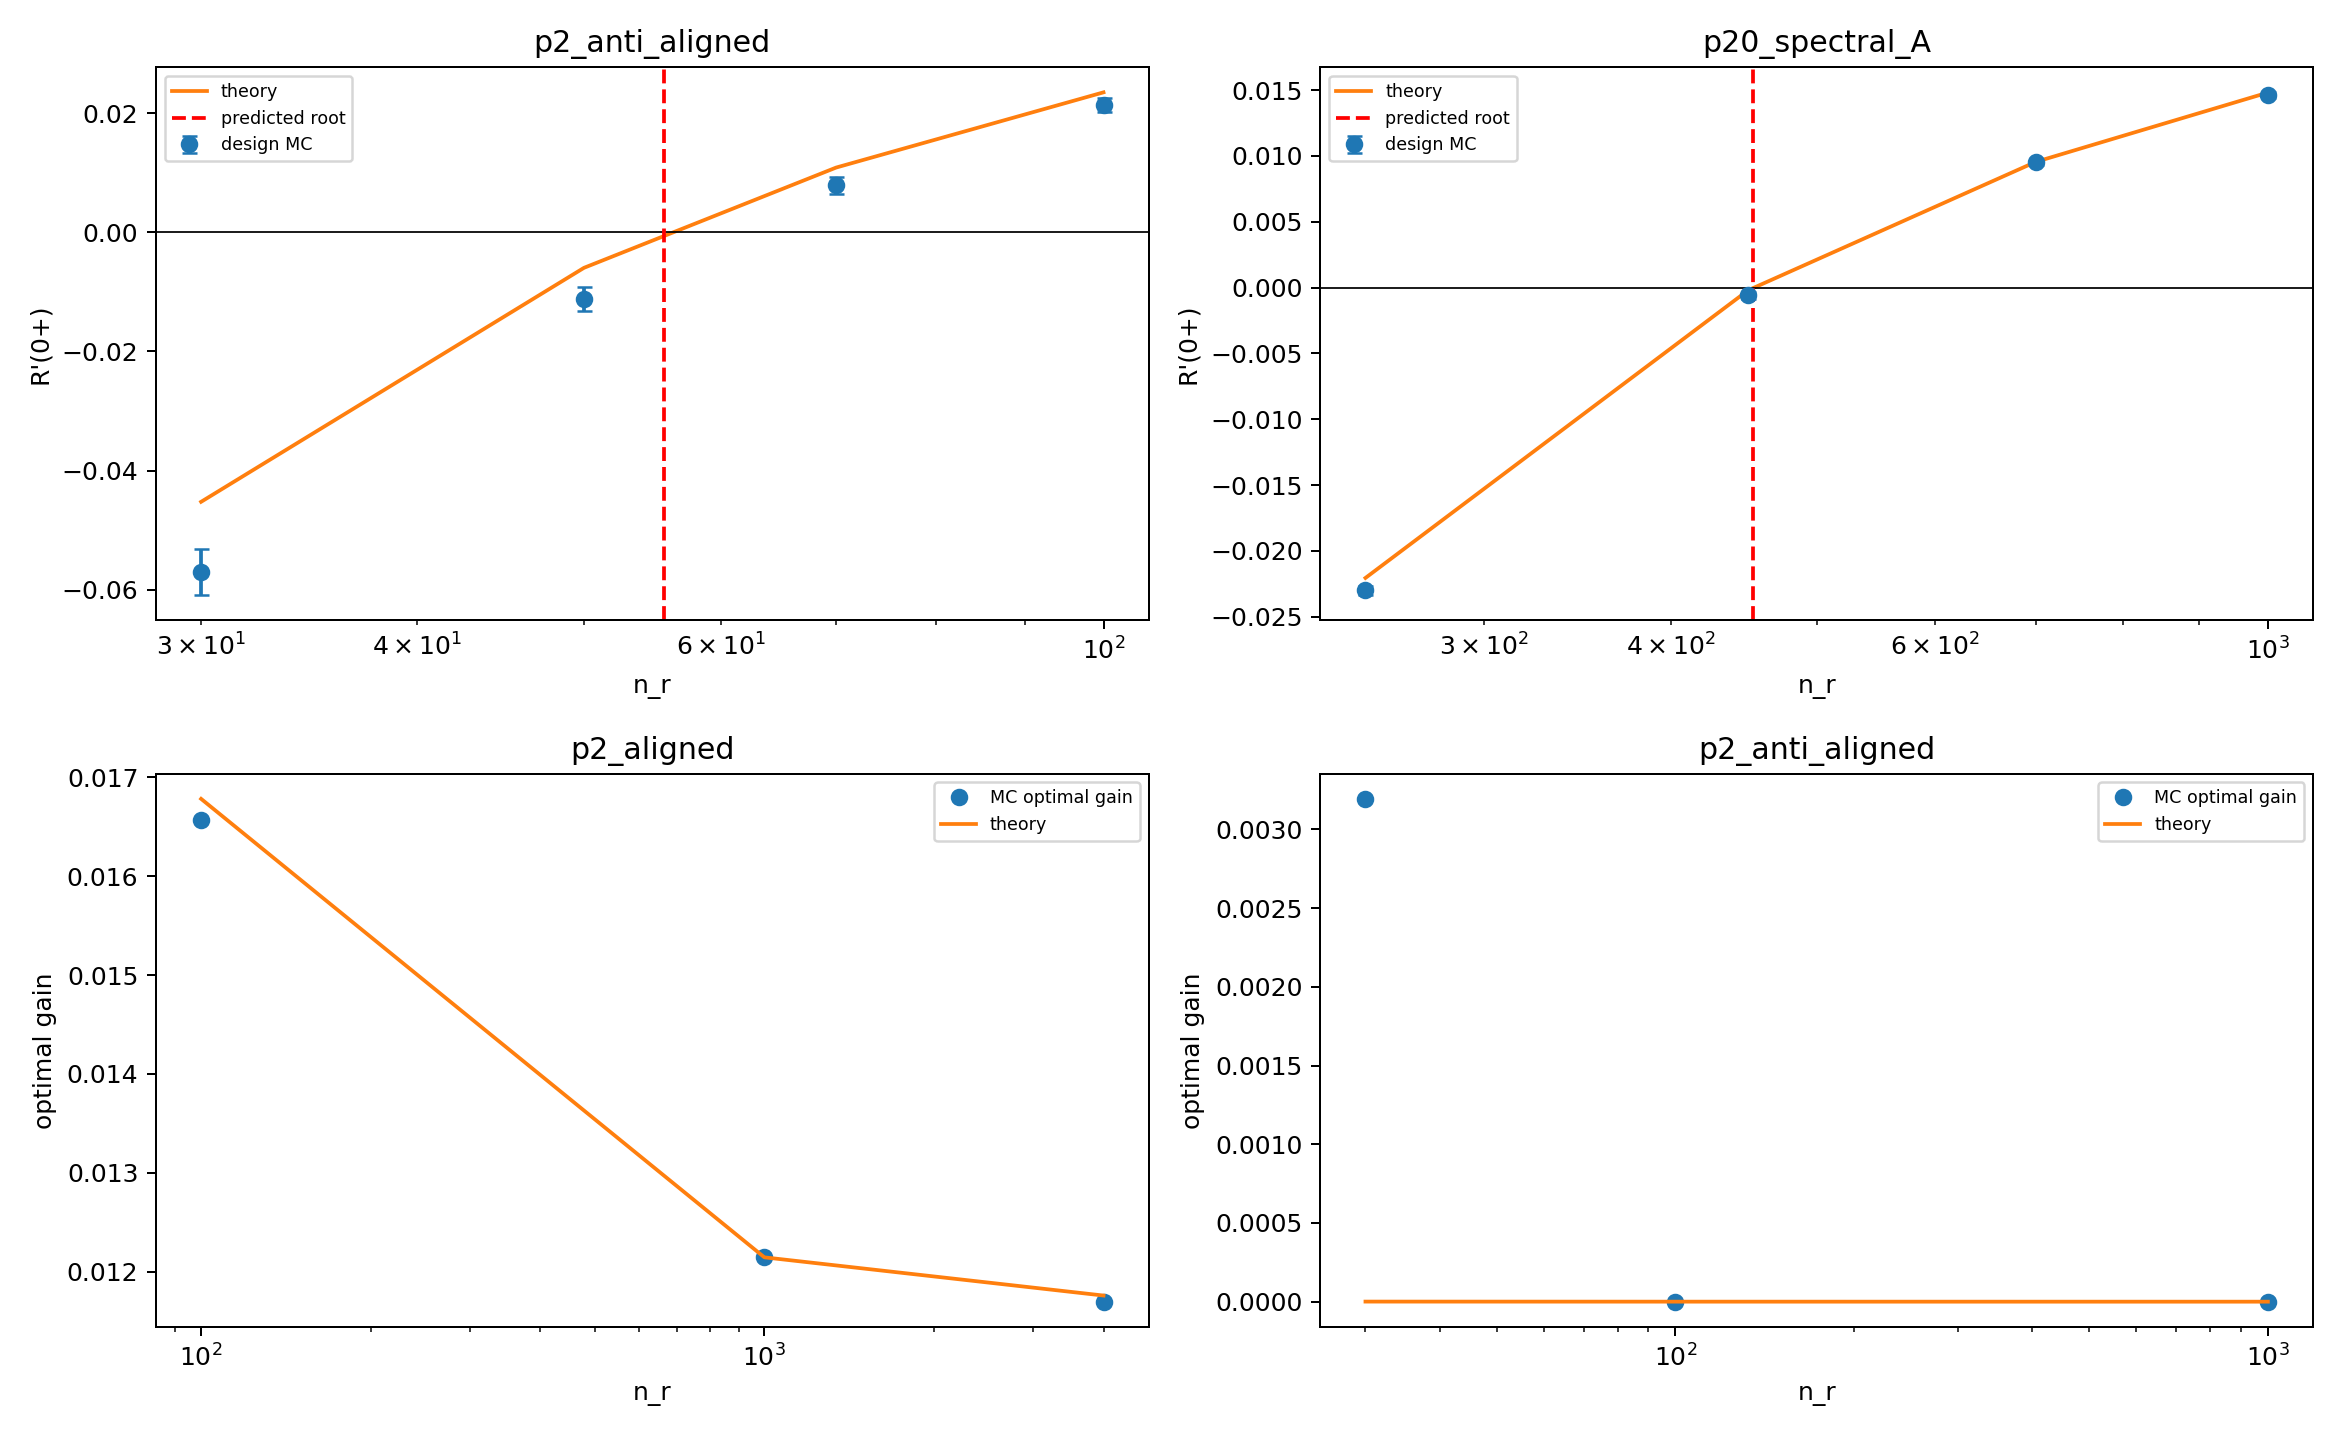
\includegraphics[width=\linewidth]{fig/s5_overview.png}
  \caption{Pre-registered direct-$n_r$ derivative and optimal-gain checks. Raw draws and bootstrap procedures are summarized in \texttt{summary.json}.}
  \label{supp:fig:s5overview}
\end{figure}

The 16 matched-dose cells compare the analytical optimum with grid minima of the same quadratic surrogate, with maximum gain discrepancy $1.49\times10^{-10}$ and a surrogate crossing to $w=1$ at $\nh=1779.17$. They verify the implementation of the surrogate formula. Exchange checks concern the first-order equation, including no-finite-solution cells at $\nr=1000$ and a finite algebraic example $\kex^{(1)}=2.8527963$ at $\nr=40,\rho=6$.

Flat-boundary cells preserve the original 400-replicate results and add pre-registered noise diagnostics. At $\nr=10^5$, theory gives $w=0.084335$ and gain $1.361\times10^{-6}$; high-repetition Monte Carlo gives $w=0.073090$ and gain $(1.214\pm0.159)\times10^{-6}$. At $\nr=10^6$, the values are $w=0.008433$ and $1.361\times10^{-8}$ versus $w=0.007871$ and $(1.238\pm0.173)\times10^{-8}$. These are compatible with the asymptotic rates. The $\nr=10^4$ cell remains nonlocal and is not reported as a uniform-fit success.

\begin{figure}[t]
  \centering
  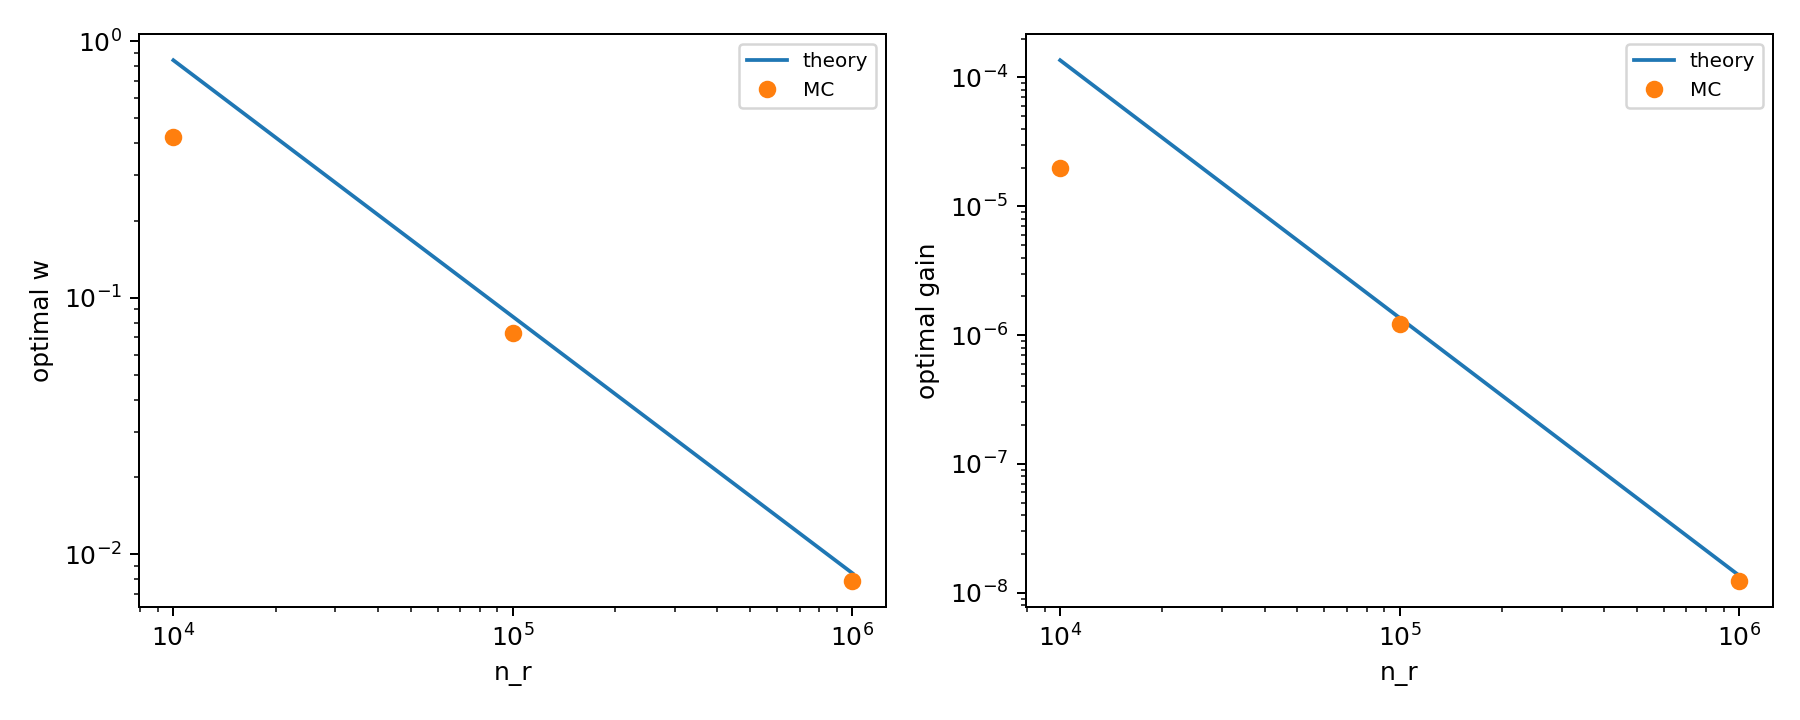
\includegraphics[width=\linewidth]{fig/s5_flat_boundary.png}
  \caption{Flat-boundary optimal weight and gain on logarithmic axes. High-repetition diagnostics reduce argmin noise without changing the preregistered criterion.}
  \label{supp:fig:s5flat}
\end{figure}

All S5 evidence is controlled-model evidence. It does not address nonlinear policies, real visual features, tuned regularization, or arbitrary non-unimodal classification.

\section{Experimental details for the trained-model validation}
\label{supp:exp}

\textbf{Generator.} Gaussian covariates with power-law spectra in a shared (rotatable) eigenbasis; $\beta^*_j \propto j^{-(s+1/2)}$ with $s=1$ normalized to the ellipsoid $\sum_j j^{2s}\beta_j^{*2}=1$; $\sigma_r^2=1$, $\sigma_h^2=4$; $p=1000$; $\nr=1000$, $\nh=6000$ unless stated; $\mu=0.05$; spectral family A $(\alpha_r,\alpha_h)=(2.0,0.9)$, family B $(1.2,1.0)$; mismatch shapes low-frequency $j^{-1}$, white $j^0$, high-frequency $(j/p)^2$, negated for the anti-aligned regime ($c<0$).
Because $\beta^*$ is known exactly, target-domain excess risk is computed without proxies.

\textbf{Estimator ladder.} E1: diagonal ridge, closed form (200 replicates). E2: full ridge, closed form with per-sample mixture weights (200 replicates). E3: linear model trained by full-batch Adam ($\mathrm{lr}=3\times10^{-3}$, 20k steps, cosine decay, zero init), loss $\sum_i w_i(y_i-x_i^\top\beta)^2 + \mathrm{l2}\,\|\beta\|^2$ so that $\mu_{\mathrm{eff}}=\mathrm{l2}$ by construction ($\mathrm{l2}=0.05$; N1e uses optimizer-level weight decay instead); single seed in this coarse pass. E4: two-layer MLP (width 512, ReLU), Adam $\mathrm{lr}=10^{-3}$, batch 512, 5k steps, explicit $L_2$ on weight matrices; risk on a 50k-sample Monte-Carlo test set; single seed.

\textbf{Per-experiment outcomes (coarse pass).}
N1a (bridge): E1 vs.\ formula 0.150\%, E2 vs.\ the numerical surrogate $\mathrm{MSE}^{\mathrm{full,num}}$ 0.766\%, full-batch-Adam E3 vs.\ E2 $10^{-15}$ (median, an optimizer--objective identity check), E4 $\sim$32\% (single-seed report only).
N1b (uncontrolled location contrast): sign agreement 9/9 (E2), 8/9 (E3), 9/9 (E4, exploratory single seed); the low/high-frequency contrast is retained as an uncontrolled observation, not as independent location evidence.
N1c (dosage): hyperbolic fit wins the initial comparison ($R^2=0.99701$ vs.\ $0.99346$ exp, $0.98502$ log) after extending $\nh$ to $\approx 8\times$ the half-saturation point; fitted half-saturation $3331$ vs.\ theory $3865$; the pre-registered strict $1/g$-linearity gate \textbf{fails} ($R^2=0.92571<0.995$), so exact dosage linearity is unconfirmed.
N1d ($H$ boundary): global truncated-gain sign agreement with the finite-$\nr$ criterion 26/27 for E2 and E3 (not a direct zero-derivative test); point-boundary gates \textbf{fail} (E2 $0.30$, E3 $0.75$ vs.\ marginal root $0.382$), while the sign-change bracket is $[0.25,0.30]$; benefit magnitude $\sim 2\times10^{-5}$ is below the $\sim 5\times10^{-5}$ noise floor.
N1e (scalar ridge inversion): in the two tested linear configurations, $L_2$-coupled Adam gives $\mu_{\mathrm{eff}}=\mathrm{wd}/2$ at the two measured nonzero wd values; decoupled AdamW gives small inverted coefficients ($\mu_{\mathrm{eff}}\approx2.5\times10^{-7}$--$3.8\times10^{-7}$ across $\mathrm{wd}\in[0,10^{-2}]$), with residuals $\sim10^{-5}$ in configuration A and $8.24\%$ in configuration B.
This is a fitting diagnostic, not evidence that AdamW provides essentially no regularization; sensitivity to learning rate, training duration, parameter scale, and seeds is untested.
N1f (basis rotation): for E2, median formula error grows from $0.96\%$ to $30.5\%$ over $\theta=0^\circ\to90^\circ$ (doubling at $15^\circ$), with no benefit-sign flip in the tested grid; E3 already has a sign flip at $\theta=0^\circ$, so no sign-robustness claim is made for E3.

\textbf{Independent within-model E1 checks (pre-registered, fresh seeds).}
N1d-new directly estimates $R'(0^+)$ from six near-zero mixing ratios on E1 (400 replicates), rather than substituting a global truncated-gain sign.
The derivative-versus-mismatch root is $0.3756$ with joint-bootstrap 95\% CI $[0.3286,0.4288]$, containing the finite-$\nr$ theoretical root $0.3821$; the CI half-width is $13.1\%$ of the theory value, so the pre-registered compatibility gate is \textbf{PASS}. CI inclusion is not an equivalence test or external validation.
N1c-new uses 400 fresh replicates at each of 11 human sample sizes and a zero-parameter E1 dosage curve with per-coordinate feedthrough.
The measured gains are compatible with that curve ($\chi^2=11.124$, df $=11$, $p=0.433$), meaning no significant departure is detected rather than equivalence being proved; the half-saturation estimate is $3541$ (95\% CI $[2948,4243]$) versus $3624$ theoretically, and the saturation gain is $0.003724$ (CI $[0.003491,0.003992]$) versus $0.003662$.
Shapes fit only for $\nh\le4000$ give held-out RMSE $3.51\times10^{-4}$ (hyperbola), $3.83\times10^{-4}$ (logarithmic), and $8.64\times10^{-4}$ (exponential); this is a limited three-point shape comparison, not external validation.
These checks concern E1 and the leading-order risk; they do not establish migration to E2/E3.

\begin{figure}[t]
  \centering
  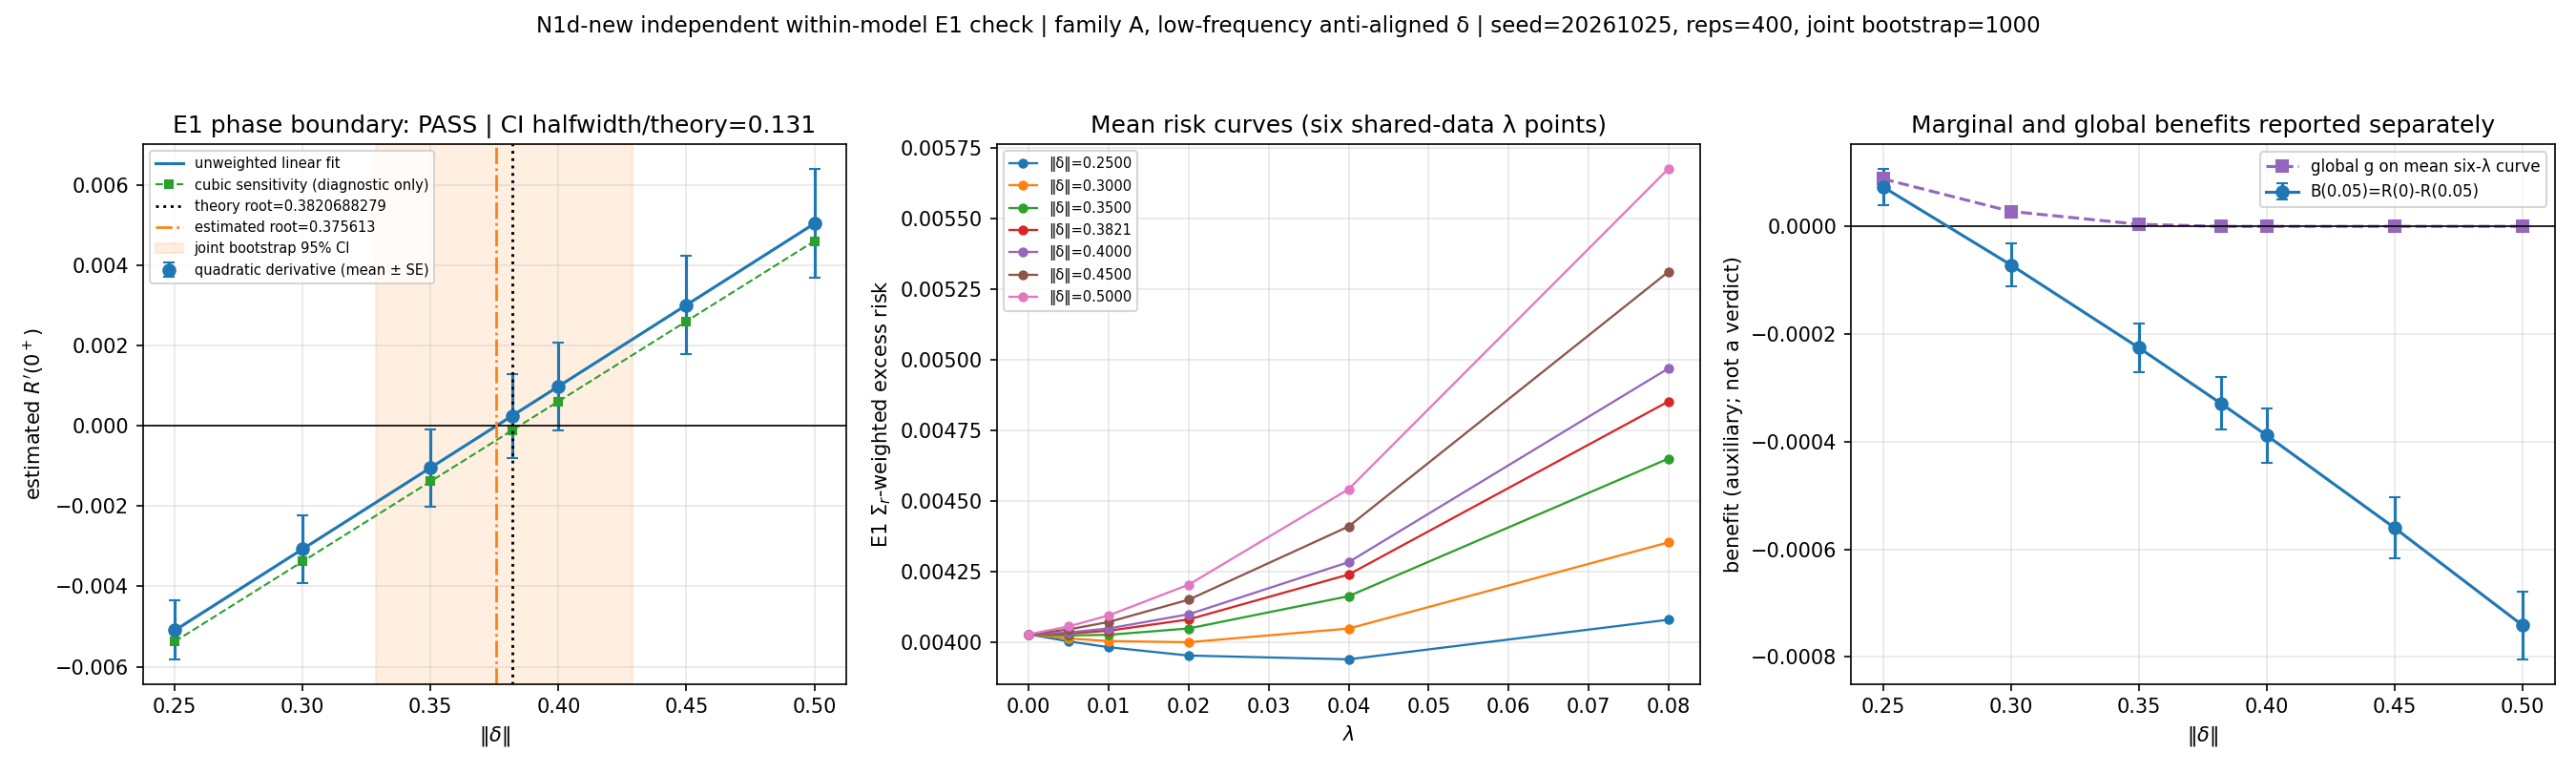
\includegraphics[width=\linewidth]{fig/n1d_e1_independent.png}
  \caption{\textbf{Independent within-model E1 phase-boundary check.} Left: direct estimates of $R'(0^+)$ versus mismatch norm, with the theoretical root inside the joint-bootstrap 95\% CI. Center: near-zero mean risk curves. Right: fixed-$\lambda$ and global gains are reported separately and do not enter the verdict. This is same-model compatibility evidence, not external or equivalence validation.}
  \label{supp:fig:n1d-e1}
\end{figure}

\textbf{Controlled mismatch experiment (constructive candidate family).}
With $\|\delta\|$, $\delta^\top\Sigma_r\delta$, and $c$ fixed, 21 controlled directions have maximum constraint residual $3.33\times10^{-16}$.
At $E=10^{-4}$, all directions have $H<0$ (range $[-4.052\times10^{-4},-1.517\times10^{-4}]$); at $E=10^{-2}$, all have $H>0$ (range $[2.420\times10^{-3},4.502\times10^{-3}]$), corresponding to $n_r^{crit}=3154$--$5870$.
At $E=10^{-6}$ the feasible set is a single point, so no location comparison is possible.
No sign flip occurs in any nondegenerate configuration: the supported conclusion is \emph{amplitude variation, not an independent location-driven phase transition}.
The extrema are selected within the disclosed constructive candidate family, not certified as global extrema.
E1 independently checks three representative directions at $E=10^{-4}$ (400 fresh replicates): derivative means are $-0.01396$, $-0.01378$, and $-0.01373$, with all bootstrap 95\% CIs below zero, consistent with $H<0$ and the finite-$\nr$ correction.
No sample-size bracketing for a quantitative $n_r^{crit}$ claim is performed.

\begin{figure}[t]
  \centering
  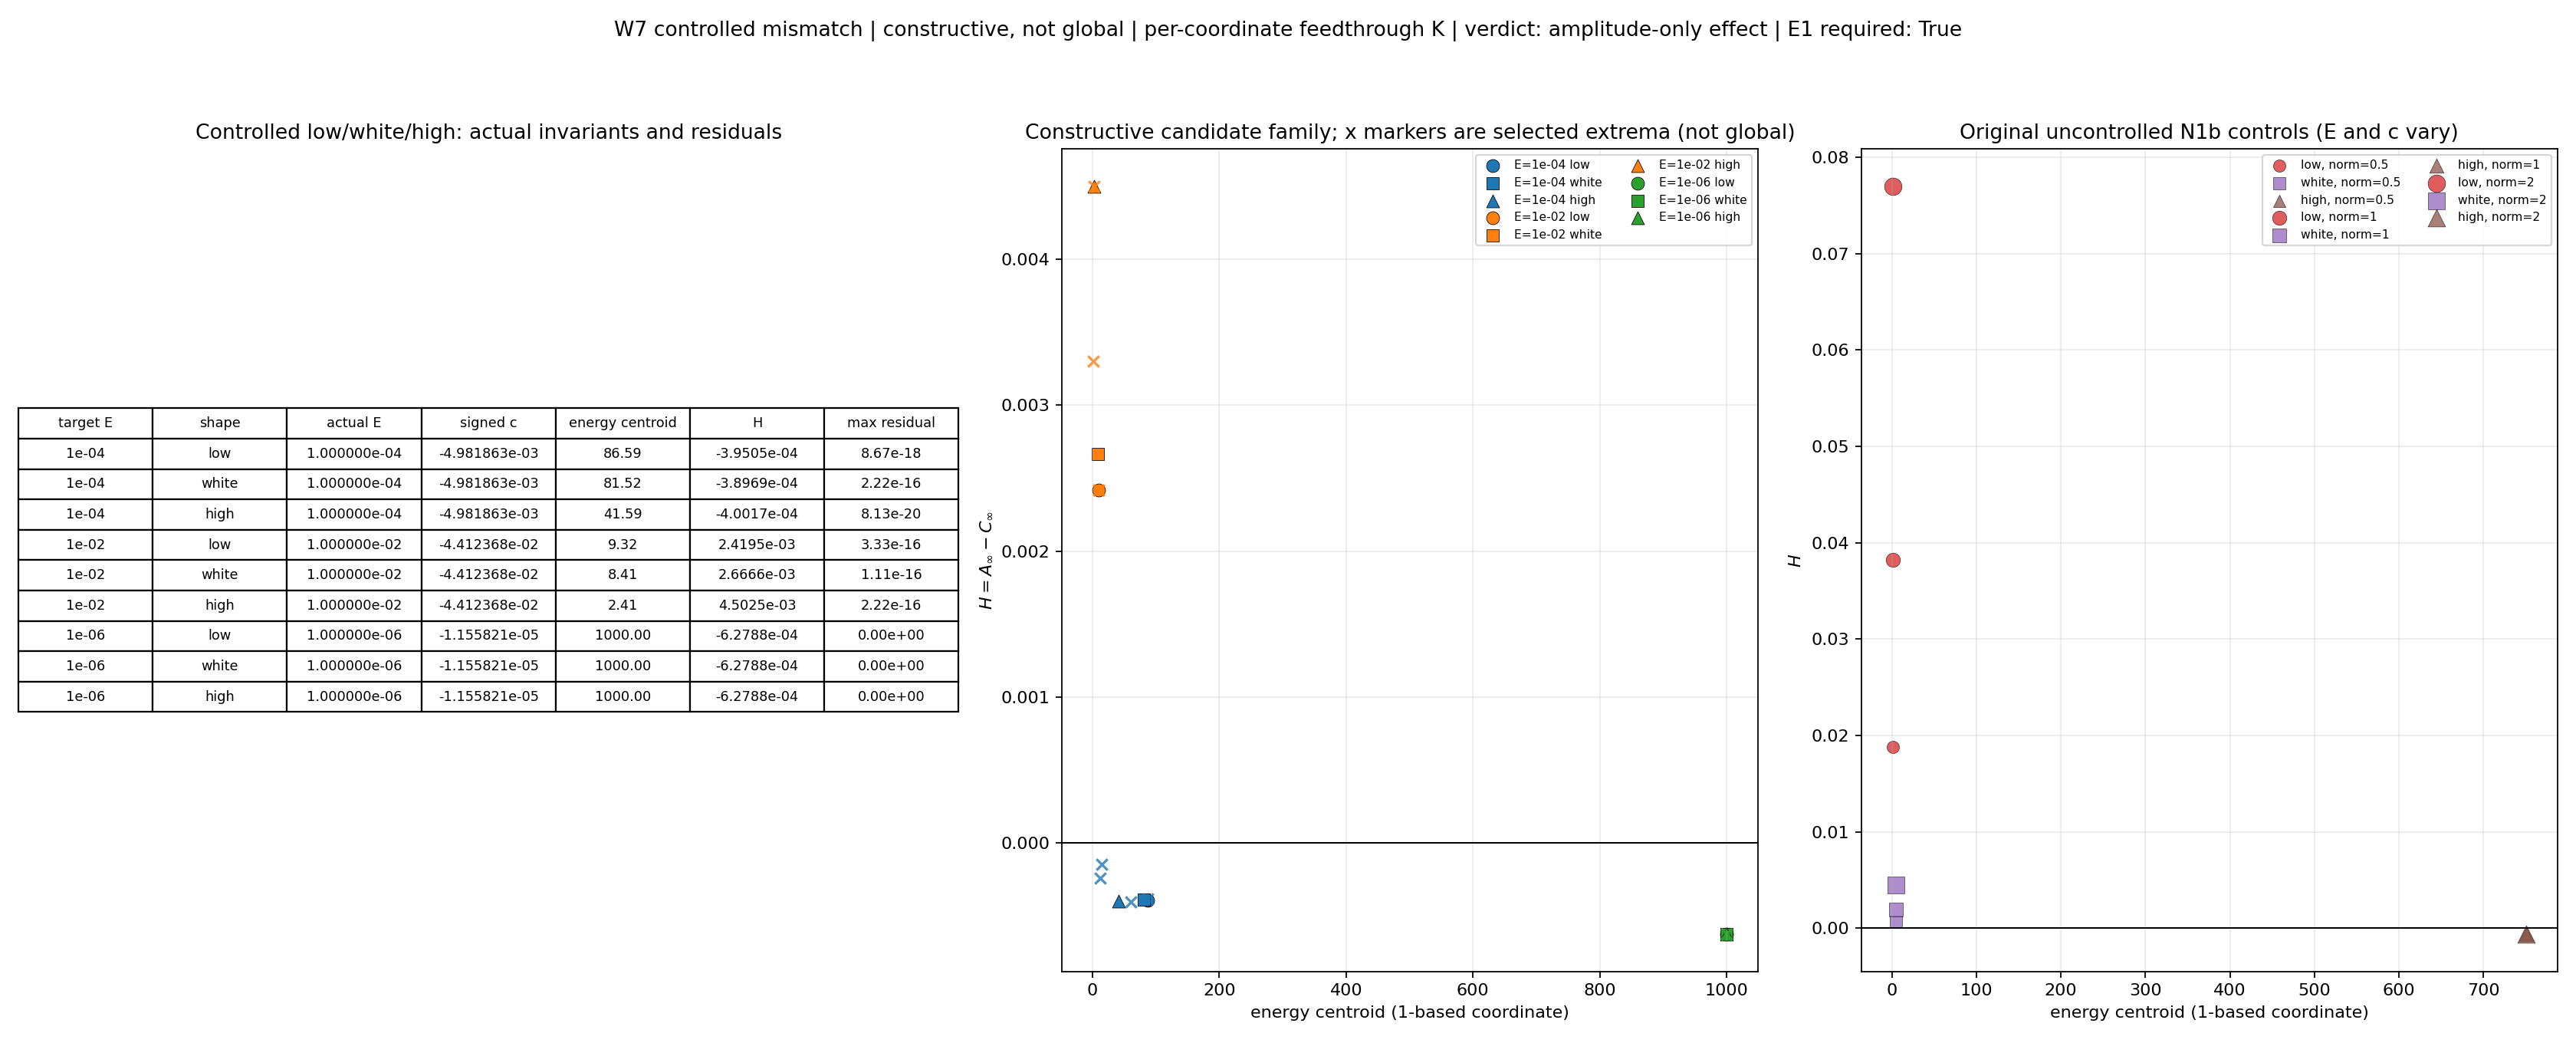
\includegraphics[width=\linewidth]{fig/controlled_mismatch.png}
  \caption{\textbf{Controlled mismatch comparison.} Left: actual invariants and residuals for the controlled low/white/high directions. Center: $H$ versus energy centroid within the constructive candidate family; no sign flip. Right: the original uncontrolled comparison in which energy and alignment also vary. The candidate-family extrema are not global-extremum claims.}
  \label{supp:fig:controlled-mismatch}
\end{figure}

\subsection{CIFAR real-feature protocol}
\label{supp:cifar-protocol}

\textbf{Features and domains.} CIFAR-10 Python batches are decoded in channel-first layout $(N,3,32,32)$. Grayscale images are the unweighted mean over the RGB channel axis. A 32-component PCA basis and feature mean are fitted on the 50{,}000 CIFAR training images only; the official test batch is reserved for final evaluation. Target samples come from classes 0--4 and auxiliary samples from classes 5--9. The original class labels are used only to define these domains, not as regression targets.

\textbf{Controlled labels.} The target regression vector has ten nonzero entries, $\beta^*_j=s_jj^{-1/2}$ for $j=1,\ldots,10$, with fixed random signs $s_j\in\{-1,1\}$. Mismatch directions are $j^{-1}$, constant, and $(j/p)^2$ for the low-frequency, white, and high-frequency arms, respectively. Each direction is normalized to $\|\delta\|=0.5$ and negated when necessary to make $\beta^{*\top}\delta\leq0$. Target and auxiliary labels are $x^\top\beta^*+\varepsilon_r$ and $x^\top(\beta^*+\delta)+\varepsilon_h$, with noise variances 1 and 4. We use $\nh=6\nr$, $\nr\in\{50,100,200,500,1000,2000\}$, 200 replicates for the low-frequency arm, and 50 for each other arm.

\textbf{Validation and test separation.} Each target replicate is split in random order into 80\% fitting and 20\% validation samples. Candidate values are $\mu\in\{0.001,0.01,0.05,0.1,0.2\}$ and $w\in\{0,0.05,0.1,0.2,0.4,0.5,0.7,1\}$. For every $w$, $\mu$ is selected by minimizing mean squared error between model predictions and the noisy target validation labels. The selected $w$ minimizes the same validation-label criterion across the resulting optimally tuned candidates; equivalently, the reported selection is the joint minimum over the $(\mu,w)$ grid. Target-only and fixed-$w=0.5$ baselines receive their own validation-selected $\mu$. Neither $\beta^*$ nor test data enters any selection step. After selection, $\beta^*$ is used only to compute noise-free target excess risk on the held-out CIFAR test features. Separately labelled oracle test-grid gains compare independently test-minimized target-only and mixed grids; they are diagnostic upper bounds, not validation-selected decisions.

\textbf{CIFAR-MLP calibration.} The additional low-frequency MLP arm uses $\nr\in\{100,500,1000\}$, width 32, 500 Adam steps, and $L_2\in\{0,10^{-4},10^{-3}\}$. Target-only L2 calibration averages noisy validation-label MSE over two seeds, using the same 80/20 split convention, and final test risks are reported over five evaluation seeds. Test features and $\beta^*$ do not participate in L2 selection.

\textbf{Aggregation conventions.} For the coarse synthetic sweeps above, benefits are computed on the estimator's risk curve ($R(0)-\min_\lambda R(\lambda)$), not by taking per-replicate minima before averaging (which incurs a Jensen bias); single-seed artifacts are flagged per cell in the JSON outputs. For CIFAR, validation selection is instead performed independently within each replicate before averaging gains, matching the deployable decision procedure; error bars show 1.96 standard errors.

\textbf{Compute.} CPU only; closed-form 200-replicate sweeps take minutes; the full coarse batch of Adam-trained arms takes a few hours on one workstation.

{
    \small
    \bibliographystyle{ieeenat_fullname}
    \bibliography{main}
}

\end{document}
